\documentclass[11pt]{report}
% Packages (Easier to list here than to use mystyle.sty)
\usepackage{graphicx}
\usepackage{tabularx}
\usepackage[margin=1.05in]{geometry}

\usepackage{amsmath} % math stuff
\usepackage[version=4]{mhchem} % Chem. equations
\usepackage{siunitx} % SI units
\DeclareSIUnit\torr{torr}
\sisetup{range-phrase=-}
\sisetup{range-units=single}

\usepackage{miller} % for formatting miller indices

\usepackage{caption} % Captions have smaller margins
\usepackage{subcaption} % for subfigures, e.g. a and b
\usepackage{booktabs} % prettier tables
\usepackage{setspace} % for double spacing
\usepackage{kpfonts} % nice font

\usepackage[hidelinks]{hyperref} % Add clickable TOC, and clickable equation refs
\usepackage{tocloft}
\setlength\cftaftertoctitleskip{5pt}

% Once I have a .bib, uncomment this
\usepackage[backend=bibtex,style=nature,url=false,doi=false,isbn=false, intitle=true, articletitle=false, eprint=false]{biblatex}
\usepackage{breakcites} % Allows citation to break into lines in bibliography
% Select the bibliography file.  I don't care at months and days
\bibliography{MS_thesis.bib}
\AtEveryBibitem{\clearfield{month}}
\AtEveryBibitem{\clearfield{day}}

%% Change the tableofcontents title
\renewcommand{\contentsname}{Table of Contents}
\hyphenation{super-exchange}

%% Macros
% Make vectors bold instead of arrows
\let\vec\mathbf

\begin{document}
\pagenumbering{roman} 
    %!TEX root = ../main.tex

\begin{center}
        % \vspace*{1cm}
 
        \textbf{The Impact of Oxygen Octahedral Rotations on Magnetism in Complex Oxide Bilayers}\\
        \vspace{.5cm}
        by\\
        \vspace{.5cm}
        NOLAN JUDD AHLM\\
        THESIS\\
        \vspace{.5cm}
        Submitted in partial satisfaction of the requirements for the degree of\\
        \vspace{.5cm}
        MASTER OF SCIENCE\\ 
        \vspace{.5cm}
        in\\
        \vspace{.5cm}
        Materials Science and Engineering\\
        \vspace{.5cm}
        in the\\
        \vspace{.5cm}
        OFFICE OF GRADUATE STUDIES\\
        \vspace{.5cm}
        of the\\
        \vspace{.5cm}
        UNIVERSITY OF CALIFORNIA\\
        \vspace{.5cm}
        DAVIS\\
        \vspace{.5cm}
        Approved:\\
        \vspace{1cm}

        $\rule{9cm}{0.15mm}$\\
        Yayoi Takamura, Chair\\
        \vspace{1cm}
        $\rule{9cm}{0.15mm}$\\
        Roopali Kukreja\\
        \vspace{1cm}
         $\rule{9cm}{0.15mm}$\\
        Apurva Mehta\\
        \vspace{.5cm}
        Committee in Charge \\
        \vspace{.5cm}
        2020


\end{center}

    %!TEX root = ../main.tex


\begin{center}
The Impact of Oxygen Octahedral Rotations on Magnetism in Complex Oxide Bilayers\\
\vspace{2cm}
\textbf{Abstract}
\end{center}
\begin{doublespace}
Complex oxides are a unique class of materials that possess a wide range of functional properties that are highly tunable as a result of the interplay between spin, charge, orbital, and lattice degrees of freedom.  
The complex nature of the interactions between different degrees of freedom leads to novel interfacial behavior and a rich parameter space with interesting functionalities.  
Bilayers of \ce{La_{0.7}Sr_{0.3}MnO3} (LSMO) / \ce{La_{0.7}Sr_{0.3}CoO3} (LSCO) are a prime example of a complex oxide system displaying unique magnetic properties.  
LSMO / LSCO bilayers grown on the cubic substrate \ce{(LaAlO3)_{0.3}(Sr2TaAlO6)_{0.7}} (LSAT) exhibit charge transfer between the LSMO and LSCO layers resulting in the formation of a thin magnetic LSCO layer at the LSMO / LSCO interface.  
The interfacial LSCO layer has a high concentration of \ce{Co^2+} ions and is magnetically coupled with the LSMO layer.  

In this work, the effect of manipulating the lattice degree of freedom on magnetic behavior and charge transfer in LSMO / LSCO bilayers was investigated by growing bilayer films on the orthorhombic substrate \ce{NdGaO3} (NGO), which enhances oxygen octahedral rotations in the film.  
Because magnetic behavior is intimately linked to the bonding geometry, manipulation of oxygen octahedral rotations provides a method to manipulate magnetic behavior in complex oxides.  
The bilayers were grown using pulsed laser deposition followed by structural characterization using x-ray reflectivity and x-ray diffraction to verify structural parameters.  
Diffraction from half-order Bragg peaks was utilized to determine the octahedral rotation pattern, while diffraction simulations were used to obtain quantitative octahedral rotation angles.  
X-ray absorption (XA) was used in order to study the charge transfer phenomena, while x-ray magnetic circular dichroism (XMCD) was employed to determine magnetically active states.  
Finally, vibrating sample magnetometry was used to measure the magnetic switching behavior of the films.  

It was found that the octahedral rotation pattern of LSMO / LSCO bilayers on NGO substrates differs from both the bulk film rotation patterns as well as that of the substrate.  
XA and XMCD results showed that the charge transfer process responsible for \ce{Co^2+} ion-rich layer formation only occurs in bilayers on NGO substrates with LSCO layer thickness of \SI{4}{\nm} and below.  
Furthermore, the lack of any trend in magnetic anisotropy and switching as a function of thickness indicates that a number of competing factors are responsible for the complicated magnetic behavior present in LSMO / LSCO bilayers on NGO substrates.  
\end{doublespace}

    \newpage
    \tableofcontents
    \newpage
\newpage 
\doublespacing
\pagenumbering{arabic} 
    %!TEX root = ../main.tex
\chapter{Introduction}
Complex oxides are a unique class of materials exhibiting a large number of technologically relevant functional properties including ferroelectricity, superconductivity, and ferromagnetism ~\cite{Cohen1992,Liang1992,Rao2000}.  
These functional properties are intimately linked to the spin, charge, lattice, and orbital degrees of freedom resulting in extreme sensitivity to external stimuli, structural distortions, and chemical doping.  
Advances in thin film growth techniques have enabled the growth of epitaxial thin films with atomically flat interfaces, allowing for the creation of artificial multi-layered structures with novel interfacial behavior.  
\section{Perovskite Structure}
One class of complex oxides, the perovskites, have received a wide range of interest due to their intriguing functional properties.  
Perovskite oxides have the general chemical formula \ce{ABO3}.  
In an ideal case they can be constructed by placing a \ce{BO6} octahedron at the center of a cubic lattice and then filling the corner positions with A-site cations, resulting in a 3 dimensional network of corner sharing \ce{BO6} octahedra.  
A 2x2x2 perovskite supercell is shown in Figure~\ref{fig:perovskite_unitcell}.  
\begin{figure}[tb]
    \centering
    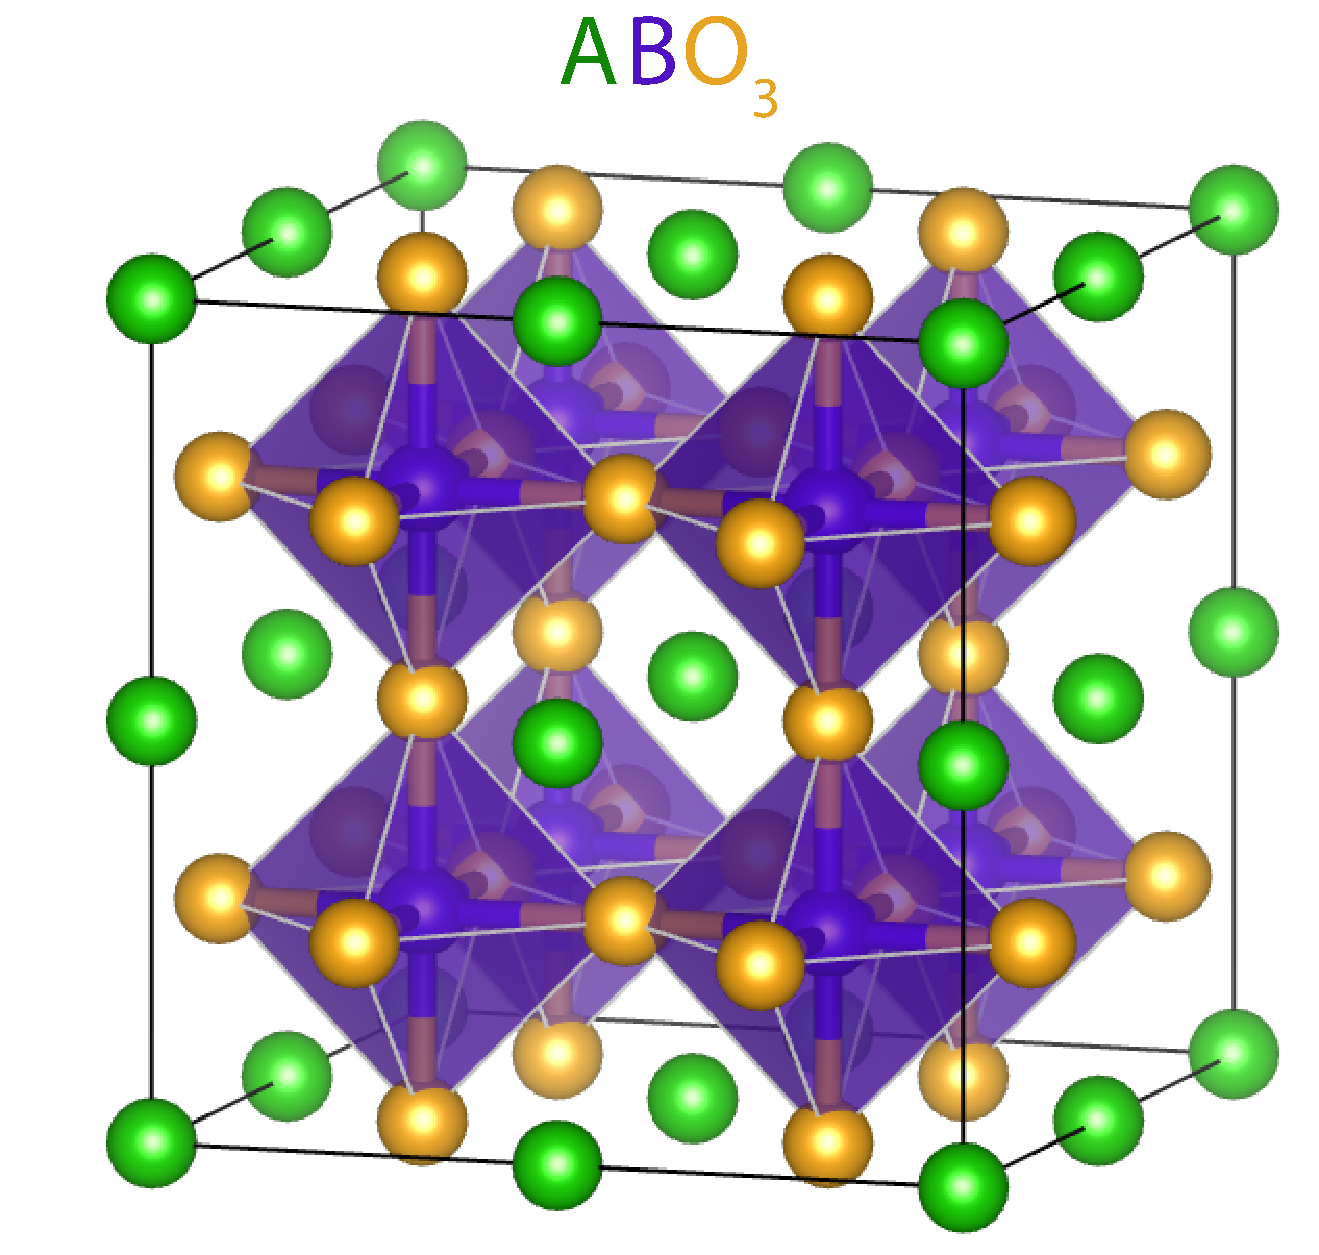
\includegraphics[width=.35\textwidth]{figures/intro/Perovskite_supercell.pdf}
    \caption[Perovskite crystal structure]{8 unit cells of the perovskite structure, illustrating the \ce{BO6} octahedra as the primary building block}
    \label{fig:perovskite_unitcell}
\end{figure}
Unique to perovskites is their ability to host nearly the entire periodic table in the various atomic positions.  
Figure~\ref{fig:intro/perovskite_ptable} depicts which atoms can be placed in the perovskite structure clearly illustrating the chemical diversity of the A and B sites.  
\begin{figure}[tb]
    \centering
    \includegraphics[width=.5\textwidth]{figures/intro/PerovskitePTable.png}
    \caption[Elements that can exist in the perovskite structure]{Color coded periodic table depicting which elements can sit in the respective positions in the perovskite crystal structure.  A-site ions are green, B-site ions are purple, and O-sites are gold. \cite{Petrovic2015}}
    \label{fig:intro/perovskite_ptable}
\end{figure}
This ability to host so many atoms is a direct result of the flexible corner shared \ce{BO6} octahedral network that is able to both distort and rotate to accommodate varying ion sizes.  
The Goldschmidt tolerance factor relates the A-O and B-O bond lengths, dictating whether or not specific A and B site ions can be accommodated~\cite{Goldschmidt1926}:
\begin{equation}
    t = \frac{r_A + r_O}{\sqrt{2}\left(r_B + r_O\right)}
    \label{eq:Goldschmidt}
\end{equation}
where $r_A$, $r_B$, and $r_O$ are the ionic radii of the various ions.  
For the ideal structure with cubic symmetry, $t=1$.  
The perovskite structure remains stable for values of $t$ ranging from 0.78 to 1.05 with symmetry lowering distortions occurring for values differing from unity, resulting in orthorhombic, rhombohedral, and hexagonal perovskite variants~\cite{Vailionis2015}.  
The tolerance factor summarizes the changing of B-O-B bond angles and bond lengths needed to accommodate larger or smaller ions and codifies the resulting crystallographic symmetry changes.  

While the Goldschmidt tolerance factor describes the resulting symmetry in a perovskite, it contains no information about the actual changes in the \ce{BO6} octahedral network.  
Changes to the B-O-B bond angle can also be described as rotations of the \ce{BO6} octahedra away from their ideal positions.  
Effort has been made to describe all of the possible rotation patterns of \ce{BO6} octahedra in perovskites, with the only constraint being the corner connectivity between octahedra.  
In the early 1970s, Glazer studied all of the possible rotation patterns and determined that there are only 23 distinct possibilities that can be described with a succinct three index notation~\cite{Glazer1972,Glazer1975}.  
Consider Figure~\ref{fig:inpahse_oop_octahedral}, which compares the $\mathrm{a}^0\mathrm{a}^0\mathrm{c}^+$ and $\mathrm{a}^0\mathrm{a}^0\mathrm{c}^-$ octahedral rotation patterns.  
\begin{figure}[b]
    \centering
    \includegraphics[width=.5\textwidth]{figures/intro/rondinelli_inphase_oophase.png}
    \caption[Depiction of in-phase and out-of-phase octahedral rotations]{Comparison of in-phase rotations (left) and out-of-phase rotations (right) about the c-axis.  \cite{Rondinelli2012}}
    \label{fig:inpahse_oop_octahedral}
\end{figure}
In this notation, each index refers to rotations about the three principle axes and the superscript denotes whether the rotations are in-phase (+), out-of-phase (-), or non-existent (o).  
If two indices have the same letter that means that the rotation magnitude is equal around those two axes.  
Figure~\ref{fig:inpahse_oop_octahedral} depicts the difference between in-phase and out-of-phase octahedral rotations.  
If the rotations are out-of-phase, the sign of rotation changes in each unit cell, whereas it remains the same for in-phase rotations.  
Two of the most common octahedral rotation patterns are the rhombohedral $\mathrm{a}^-\mathrm{a}^-\mathrm{a}^-$ pattern occurring due to ordered rotations about the [111] direction, and the orthorhombic $\mathrm{a}^-\mathrm{b}^+\mathrm{a}^-$pattern caused by rotations about the [110] direction.  

The presence of octahedral tilts changes the overall crystalline symmetry of the perovskite structure.
It can be helpful to consider a ``pseudocubic'' (pc) set of axes and lattice parameters that correspond to the ideal perovskite perovskite building blocks.  
Transformation from an orthorhombic unit cell to a pseudocubic unit cell can be performed through a simple transformation, with the relationship between orthorhombic and low index pseudocubic directions outlined in Table~\ref{tab:ortho pc transform}.  
The pseudocubic representation in Table~\ref{tab:ortho pc transform} is just one of multiple different transformation that can be used for orthorhombic unit cells.  
\begin{table}[tb!]
\centering
\caption{Relationship between low index pseudocubic and orthorhombic directions for a (110) oriented orthorhombic substrate, where the listed pseudocubic directions are parallel to the original orthorhombic directions}
\label{tab:ortho pc transform}
\begin{tabular}{@{}ll@{}}
\toprule
Orthorhombic & Pseudocubic\\ \midrule
\hkl[1 1 0] & \hkl[0 0 1] \\
\hkl[1 -1 0] & \hkl[0 1 0] \\
\hkl[0 0 2] & \hkl[1 0 0] \\
\bottomrule
\end{tabular}
\end{table}


\section{Magnetism in Perovskites}
Magnetic behavior in materials is due to exchange interactions between two neighboring atoms with net magnetic moments.  
Magnetic exchange interactions are effectively a driving force minimizing energy when spins are aligned in antiparallel or parallel directions, depending on the sign of the exchange interaction.  
Multiple types of exchange interactions exist: direct exchange in which two atoms are in close proximity and interact directly with one another, and indirect exchange which requires an intermediary to facilitate the exchange interaction between separated atoms~\cite{Spaldin2010}.    
In the perovskite structure, the A site ion typically has a full shell electrical configuration and thus the magnetic behavior can be solely attributed to the B site ion.  
The large separation between neighboring B site ions requires an indirect exchange mechanism mediated by the \ce{O^2-} ions to account for any observed (anti)ferromagnetic behavior.  

Consider the perovskite \ce{La_{0.7}Sr_{0.3}MnO3} (LSMO) which consists of a mixture of La and Sr ions on the A site, and Mn on the B site, and is ferromagnetic below \SI{370}{\kelvin}~\cite{Hemberger2002}.  
A direct result of two A site ions with different valence is that the Mn ion exists with both \ce{Mn^3+} and \ce{Mn^4+} states in an equal proportion to the \ce{Sr}/\ce{La} ratio assuming complete oxygenation.  

When a transition metal such as \ce{Mn} is octahedrally coordinated with oxygen ions, overlap between the metal 3d orbitals and oxygen 2p orbitals is significant, and the energy associated with this overlap is known as the crystal-field stabilization energy (CFSE)~\cite{Rohrer2001}.  
Two d-orbitals, $d_{z^2}$ and $d_{x^2-y^2}$, point directly at the surrounding oxygen ligands and are destabilized, while the other three d-orbitals, $d_{xy}$, $d_{yx}$, and $d_{zx}$, point at the space in between atoms and become stabilized.  
As a result, the five fold degeneracy of the 3d orbitals is lifted forming a triply degenerate set of $t_{2g}$ orbitals and a doubly degenerate set of $e_g$ orbitals.  
A schematic for this splitting due to ligand field effects is shown in Figure~\ref{fig:cfse_d_orbital}.  
\begin{figure}[tb]
    \centering
    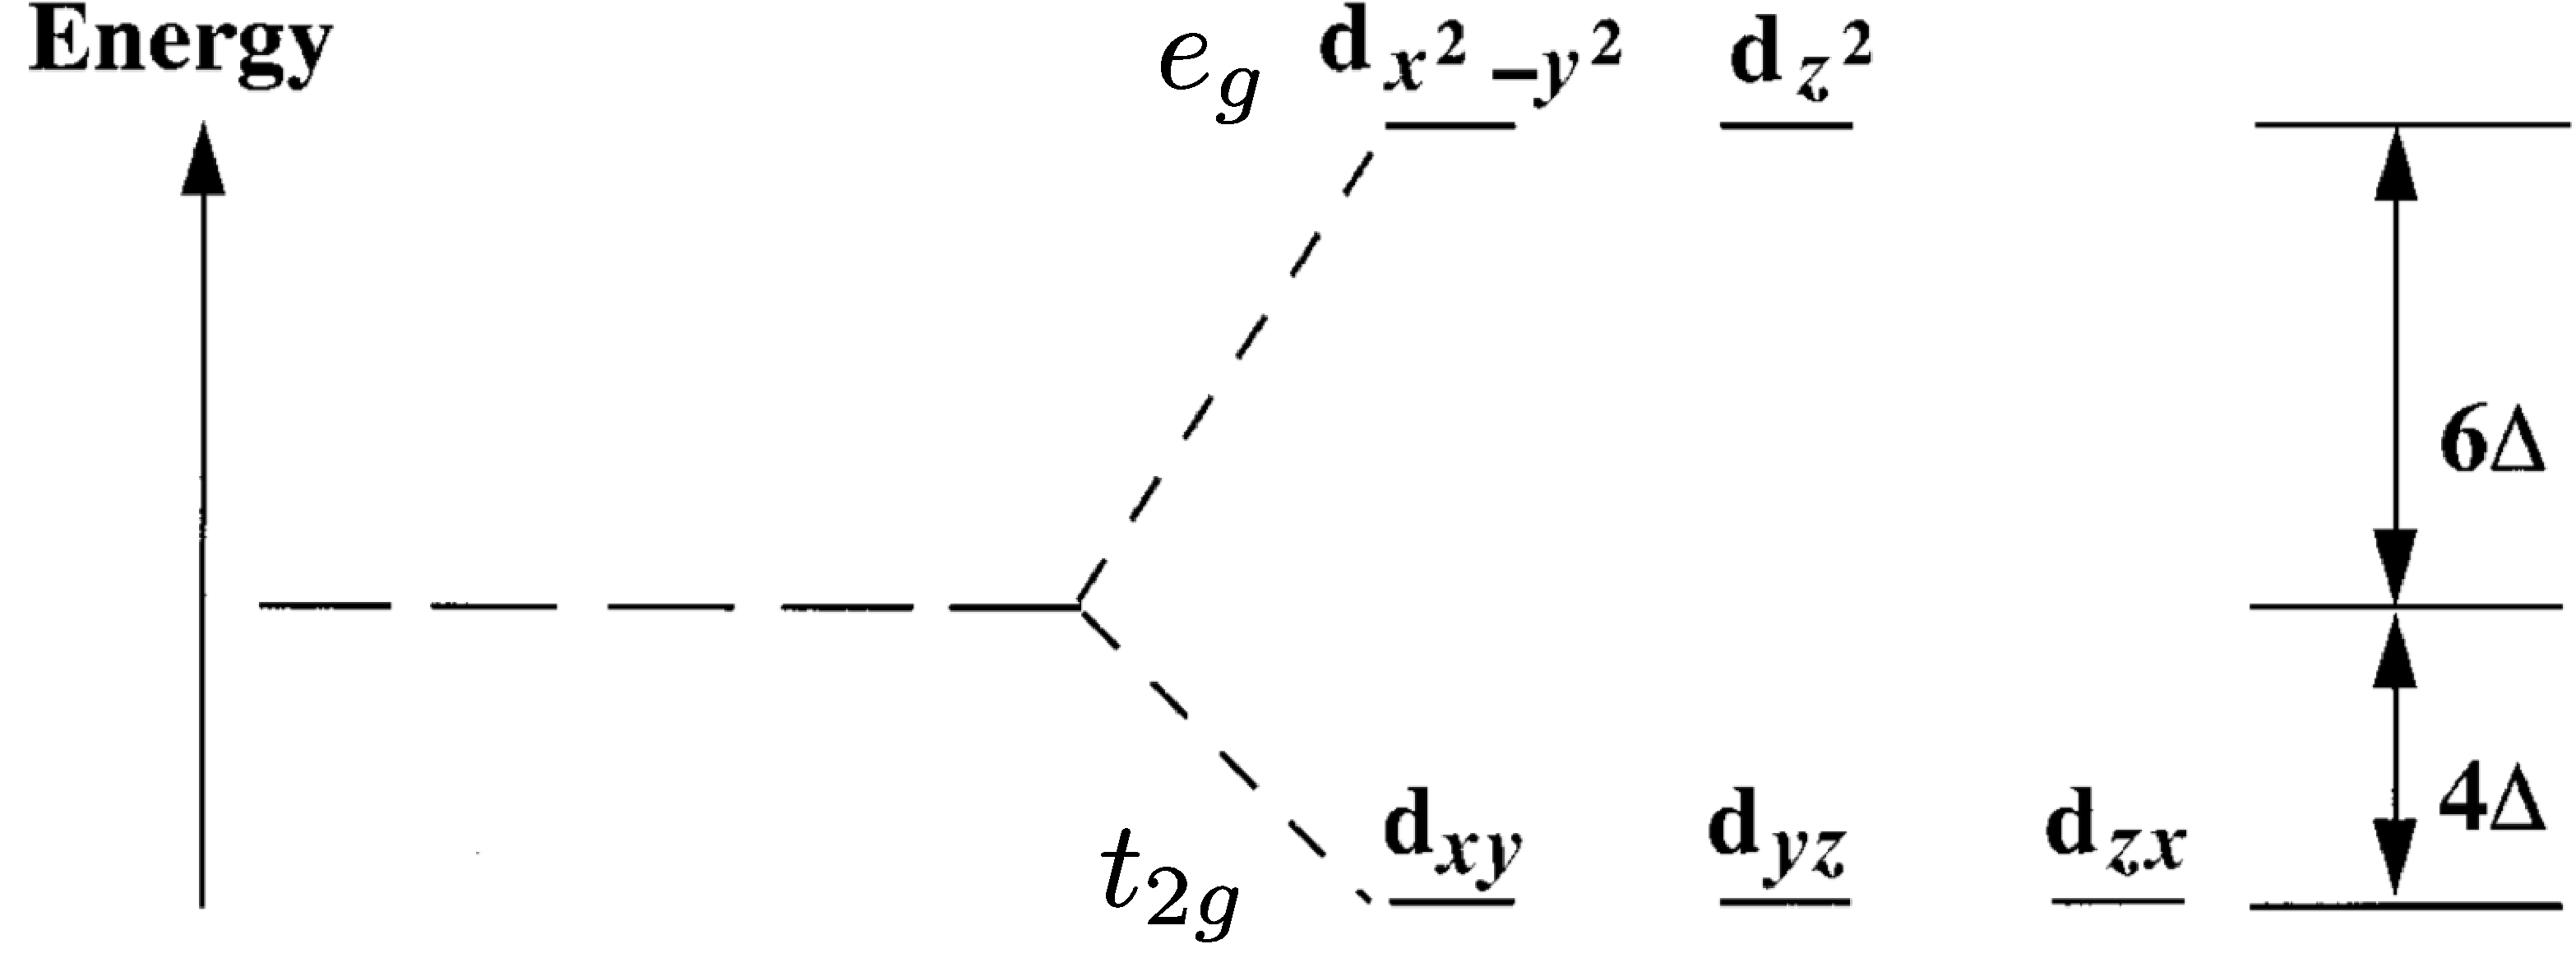
\includegraphics[width=.7\textwidth]{figures/intro/cfse_rohrer.pdf}
    \caption[Octahedral crystal field splitting of 3d orbitals]{CFSE splitting of 3d-orbitals in an octahedral bonding environment. \cite{Rohrer2001}}
    \label{fig:cfse_d_orbital}
\end{figure}
The separation between $t_{2g}$ and $e_g$ orbitals is typically on the order of 1-2 \si{\eV} in manganites, but is significantly lower for cobaltites~\cite{Fujioka2015}.  

When electrons fill the $t_{2g}$ and $e_g$ orbitals, they obey Hund's rules which state that electrons prefer to maximize the total angular momentum and total spin of an orbital.  
In other words, the lowest energy state exists when electrons fill different orbitals with parallel spin configurations.  
The case for \ce{Mn^3+} and \ce{Mn^4+} ions is illustrated in Figure~\ref{fig:Mn_double_exchange}.  
\ce{Mn} ions with different valence on either side of an intermediate O ion can now interact indirectly: first, an electron from an O 2p orbital hops onto a neighboring \ce{Mn^4+} ion followed by an electron hopping from the \ce{Mn^3+} ion to the now partially filled O 2p orbital~\cite{Zener1951}.  
Because there is an energy penalty associated with flipping electron spins, the spin direction is preserved and ferromagnetic behavior is realized.  
\begin{figure}[t]
    \centering
    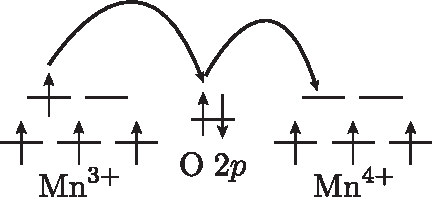
\includegraphics[width=.65\textwidth]{figures/intro/Mn_dub_exchange_schematic.pdf}
    \caption[Schematic for double exchange mechanism in LSMO between \ce{Mn^3+} and \ce{Mn^4+} ions]{Schematic for double exchange mechanism in LSMO between \ce{Mn^3+} and \ce{Mn^4+} ions.  First, an electron hops from the O 2p orbital to an empty orbital in the \ce{Mn^4+} ion maintaining spin alignment following Hund's rules.  Next, an electron hops from the \ce{Mn^3+} ion to the now partially empty O 2p orbital.  Spin direction is preserved during this hopping process, and the two ion positions have been switched.}
    \label{fig:Mn_double_exchange}
\end{figure}
Since electrons are physically hopping between neighboring ions, the onset of ferromagnetism via the double exchange mechanism is also coincident with the onset of metallic behavior.  
Furthermore, the rate and probability of electron hopping depends sensitively on the overlap between B 3d and O 2p orbitals and magnetism is therefore strongly linked with the B-O-B bond geometry and the octahedral tilt pattern.  

Another type of indirect exchange interaction that can occur in perovskites is the superexchange mechanism.  
Consider two \ce{Mn^3+} ions located on either side of an oxygen ion with a \SI{180}{\degree} bond angle, illustrated in Figure~\ref{fig:mn_superexchange}.  
\begin{figure}[h]
    \centering
    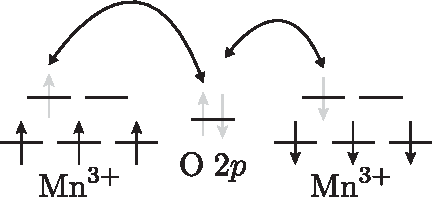
\includegraphics[width=.65\textwidth]{figures/intro/Mn_superexchange_schematic.pdf}
    \caption[Schematic for superexchange in \ce{LaMnO3}]{Schematic for superexchange in \ce{LaMnO3}.  Virtual electron hopping occurs from the O 2p orbital to neighboring Mn 3d orbitals (indicated by grey arrows).  Spin direction is preserved in this virtual hop leading to antiferromagnetic behavior.}
    \label{fig:mn_superexchange}
\end{figure}
A virtual hop from the oxygen 2p orbital to the Mn 3d orbital can occur on either side of the oxygen ion and, since the oxygen 2p orbital interacting with neighboring Mn 3d orbitals is completely filled, the electrons hopping to either Mn ion will have an opposite spin direction.  
Consequently the spin direction on the two Mn ions will be antiparallel resulting in antiferromagnetic behavior and because the hopping process is virtual the sample is insulating.  
The superexchange mechanism is dependent on orbital filling and bonding geometry: for \SI{180}{\degree} bonds the interaction is antiferromagnetic while for \SI{90}{\degree} bonds it is ferromagnetic~\cite{Bhattacharya2014}.  
The rules for determining the resulting magnetic behavior have been codified by Goodenough, Kanamori, and Anderson~\cite{Anderson1950}.  

\section{\texorpdfstring{\ce{La_{1-x}Sr_{x}MnO3}}{La(1-x)SrxMnO3} and \texorpdfstring{\ce{La_{1-x}Sr_{x}CoO3}}{La(1-x)SrxCoO3}}
Thin films and heterostructures of Sr-doped \ce{LaMnO3} and \ce{LaCoO3} will be the main focus of this work.  
Introduction of $x$ moles of the bivalent dopant Sr into either of these compounds results in the formation of an equimolar amount of \ce{Mn^4+} (\ce{Co^4+}) ions resulting in a mixed 3+ / 4+ valence state and the onset of ferromagnetism via the double exchange mechanism.  
The large number of unique phases present in the \ce{La_{1-x}Sr_{x}MnO3} temperature - doping phase diagram in Figure~\ref{fig:lsmo_phase} illustrates the complex interplay between spin, orbit, lattice, and charge degrees of freedom in this material.  
Figure~\ref{fig:lsmo_phase} also depicts the changing crystalline symmetry as the concentration of \ce{Sr} is changed: the ionic radii of Sr, \SI{1.31}{\angstrom}, is slightly larger than that of La, \SI{1.22}{\angstrom}~\cite{Shannon1976}.  
In order to accommodate this change, the \ce{BO6} octahedra rotate and the symmetry changes from orthorhombic to rhombohedral, followed by tetragonal and hexagonal symmetries as the value of $x$ increases.  
\begin{figure}[tb!]
    \centering
    \includegraphics[width=.5\textwidth]{figures/intro/LSMOPhase.png}
    \caption[\ce{La_{1-x}Sr_{x}MnO3} phase diagram]{\ce{La_{1-x}Sr_{x}MnO3} Sr-doping-temperature phase diagram.  \textbf{crystal structure} O: Jahn-Teller distorted orthorhombic, O': orthorhombic, O'': orbital-ordered orthorhombic, R: Rhombohedral, T: tetragonal, Mc: monoclinic, H: hexagonal, \textbf{magnetic order} PM: paramagnetic, CA: canted, yellow: antiferromagnetic, Blue: ferromagnetic, \textbf{electronic state} I: insulating, M: metallic.  \cite{Hemberger2002}}
    \label{fig:lsmo_phase}
\end{figure}
This work focuses on a doping concentration of \SI{0.3}{} where \ce{La_{0.7}Sr_{0.3}MnO3} (LSMO) is in a rhombohedral crystal structure and is a soft ferromagnetic metal with a low coercivity below a $T_c$ of \SI{370}{\kelvin}~\cite{Hemberger2002}.  

The doping-temperature phase diagram for \ce{La_{1-x}Sr_{x}CoO3} in Figure~\ref{fig:lsco_phase} shows similarities with that of \ce{La_{1-x}Sr_{x}MnO3}; however, distinct differences arise because \ce{La_{1-x}Sr_{x}CoO3} undergoes a phenomenon known as magnetoelectronic phase separation (MEPS) for low Sr-doping~\cite{Torija2011}.  
MEPS involves small ferromagnetic clusters that are embedded in a matrix of insulating antiferromagnetic material such that long range ferromagnetic order is not realized. 
Phase separated \ce{La_{1-x}Sr_{x}CoO3} exhibits glassy behavior and therefore this region of the phase diagram is denoted as a spin glass (SG).  
Long range ferromagnetism does not occur until the clusters grow in size and create a percolative network above $x=0.18$ upon which a metal-insulator transition occurs and long range ferromagnetism is realized.  
Furthermore the \ce{La_{1-x}Sr_{x}CoO3} phase diagram only covers doping concentrations from $x=0$ to $x=0.7$.  
At higher $x$ the perovskite structure is no longer the equilibrium phase and instead derivative structures are formed such as the oxygen deficient perovskite structure known as Brownmillerite~\cite{Jeen2013a}.  
\begin{figure}[h]
    \centering
    \includegraphics[width=.5\textwidth]{figures/intro/LSCO_Bulk_Phase_Wu2003_Labelled.eps}
    \caption[\ce{La_{1-x}Sr_{x}CoO3} phase diagram]{\ce{La_{1-x}Sr_{x}CoO3} composition - Sr-doping phase diagram.  SG = spin glass, PS = paramagnetic semiconductor, PM = paramagnetic metal, FM = ferromagnetic metal, MIT = metal-insulator transition, $T_{irr}$ = irreversiblity temperature, $T_{sst}$ = spin state transition temperature.  \cite{Wu2003}}
    \label{fig:lsco_phase}
\end{figure}
Another feature unique to \ce{La_{1-x}Sr_{x}CoO3} is the presence of spin state transitions.  
In this material the crystal field splitting between $e_g$ and $t_{2g}$ orbitals is small such that thermal energy can excite electrons from the $t_{2g}$ to $e_g$ orbitals.   
The presence of spin state transitions results in a diverse landscape of magnetic states~\cite{Wu2003}.  
The doping concentration of $x=0.3$ will be the focus of this study.  
At this Sr concentration, \ce{La_{0.7}Sr_{0.3}CoO3} (LSCO) is in a rhombohedral crystal structure and is a hard ferromagnet metal with a $T_c$ of \SI{210}{\kelvin}.  
Hard ferromagnets magnetically switch at larger fields than soft ferromagnets and typically have lower saturation magnetization.  

\section{Oxide Heterostructures}

Growing oxides into multilayered structures introduces another layer of complexity.  
The spin, charge, orbit, and lattice degrees of freedom vary dramatically across an interface and can lead to unexpected and difficult to predict physical behavior.  
One effect that occurs across an interface is the charge transfer of electrons from one material to another because of Fermi level ($E_F$) differences on either side of the interface.  
Electrons will travel into the material with the lower $E_F$ until the energy differences is equalized.  
The length scale for interfacial charge transfer is short in oxides, on the order of \SI{0.5}{\nm} to \SI{2}{\nm}, because oxides have a large dielectric constant and high carrier concentrations~\cite{Hellman2017}.  
As magnetic behavior is so closely linked with the valence state, charge transfer can drastically change local magnetic behavior.  
For example, interfacial ferromagnetism can be stabilized in nonmagnetic systems like in antiferromagnetic manganite superlattices~\cite{Santos2011} and \ce{LaNiO3} / \ce{CaMnO3} superlattices~\cite{Grutter2013}.  

Structural changes across interfaces can also influence the properties of an oxide heterostructure.  
When a thin film is grown on a substrate it can be strained depending on the relative lattice parameters and crystal structures of the substrate and thin film.  
Substrate-induced strain forces the in-plane lattice parameter of the film to match that of the substrate resulting in a tetragonally distorted film~\cite{Vailionis2011}.  
\ce{BO6} octahedral rotations are also modified by interfacial strain leading to a change in the B-O-B bond angles and a resultant impact on the magnetic behavior.  
Furthermore, \ce{BO6} octahedra are constrained to be corner connected, even across an interface, meaning that rotational patterns from a substrate can be induced into a film, providing yet another route in which magnetic behavior can be modified in oxide heterostructures.  
However, frequently, the rotation pattern observed in thin films differs both from that of the bulk material and of the substrate~\cite{Choquette2016}.  
Interestingly, the length scales over which interfacial strain and substrate induced rotational patterns persist differ~\cite{Rondinelli2012}.  

\section{LSMO / LSCO heterostructures}
\begin{sloppypar} % fixes LSAT chemical name extending to margins
Bilayers of LSMO and LSCO have been studied for their interesting magnetic switching behavior.  
When a hard ferromagnet (LSCO) and a soft ferromagnet (LSMO) are grown in a bilayer on \ce{(LaAlO3)_{0.3}(Sr2TaAlO6)_{0.7}} (LSAT) substrates, the major hysteresis loop showing the magnetization of the entire sample shows two distinct magnetic switching events~\cite{Li2014}.  
The black curve in Figure~\ref{fig:LSCO_LSMO_bilayer_loops} shows the magnetic switching behavior of a \SI{6}{\nm} LSMO / \SI{6}{\nm} LSCO bilayer on LSAT substrate.  
\begin{figure}[b!]
    \centering
    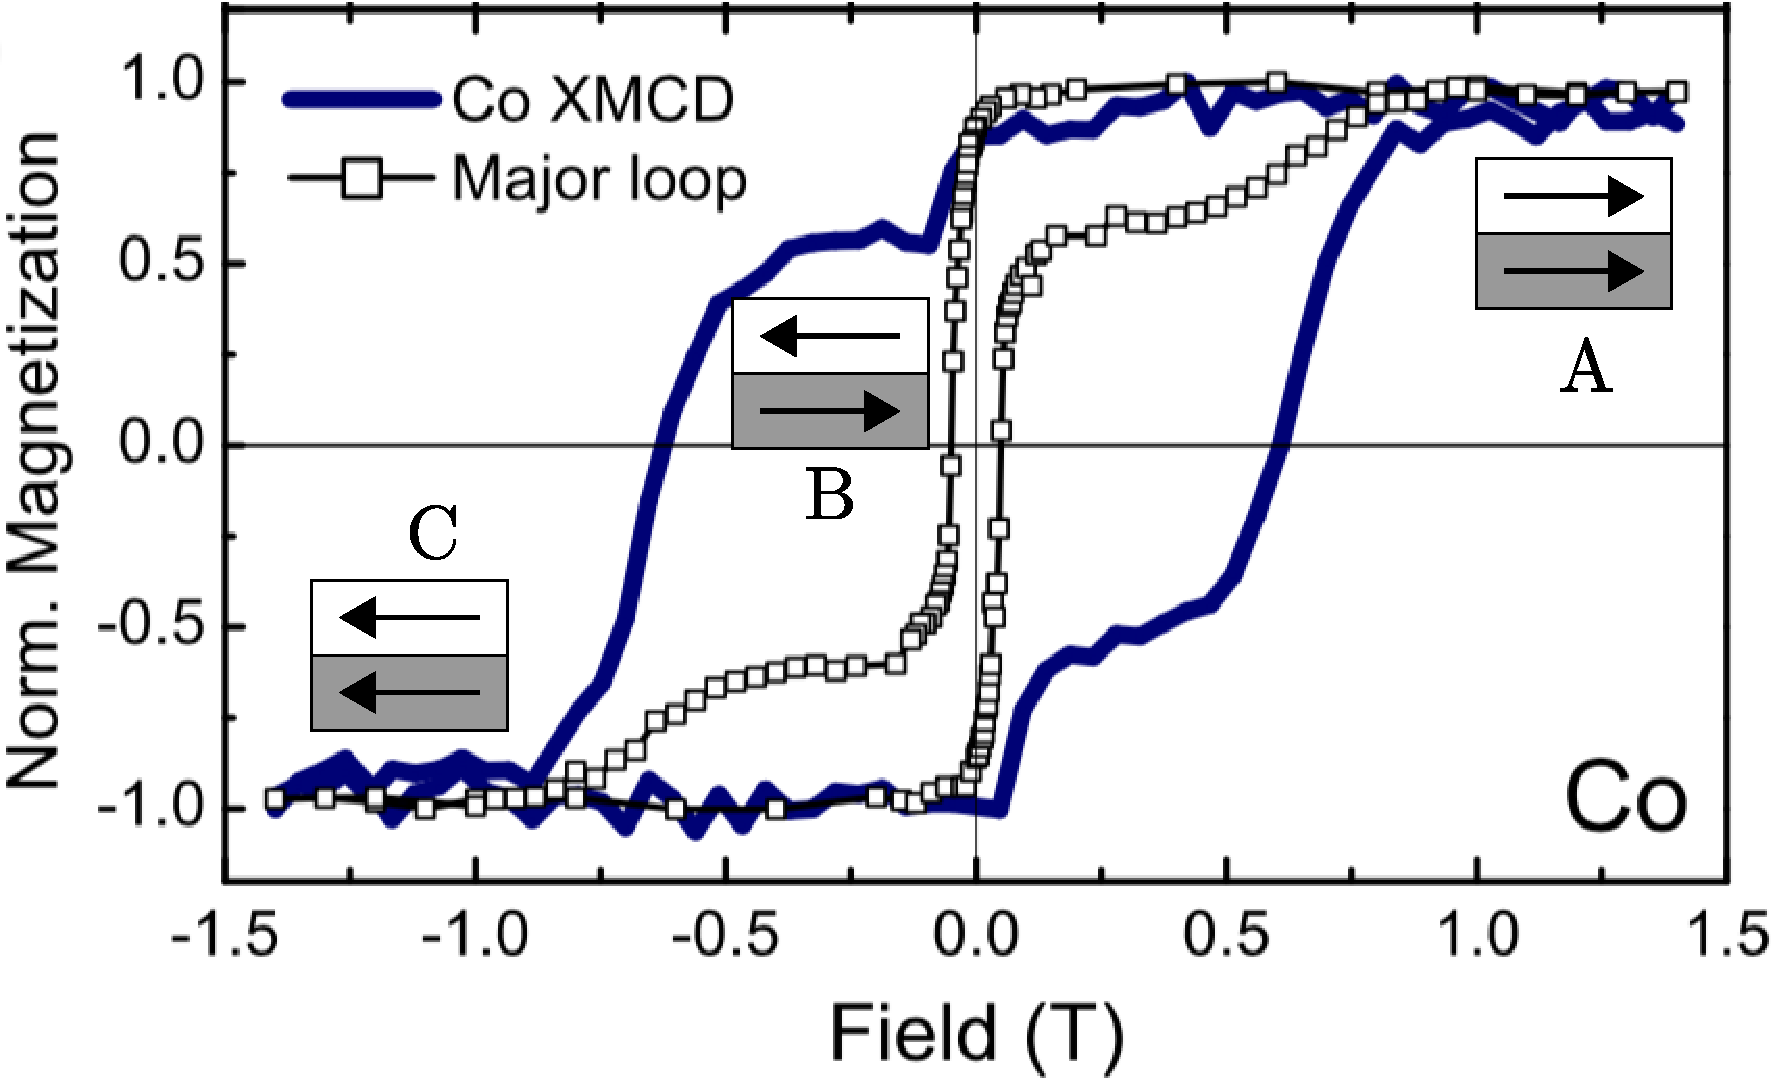
\includegraphics[width=.65\textwidth]{figures/intro/li_bilayer_loop.pdf}
    \caption[Major hysteresis loop and Co XMCD hysteresis loop for a \SI{6}{\nm} LSMO / \SI{6}{\nm} LSCO film on LSAT substrate.]{Major hysteresis loop (black) and Co XMCD hysteresis loop (blue) for a \SI{6}{\nm} LSMO / \SI{6}{\nm} LSCO film on LSAT substrate.  Arrows show directions of magnetic moments in top LSMO (white) and bottom LSCO (grey) layers.  Point A: both layers in same direction.  Point B: soft LSMO layer switches.  Point C: Hard LSCO layer switches.  From~\cite{Li2014}}
    \label{fig:LSCO_LSMO_bilayer_loops}
\end{figure}
Starting at the positive field side, the magnetization in both the LSCO and LSMO layers point in the positive direction.  
As the field is reduced, the coercive field of the soft LSMO layer is reached and its magnetization switches from positive to negative.  
The sample is now in a state where the soft layer and the hard layer are magnetized in opposite directions.  
Finally, the coercive field of the hard layer is reached and the magnetization in this layer is switched.  
The process repeats as the field is swept in the positive direction.
\end{sloppypar}
Interestingly in this bilayer system the nominally hard LSCO layer has a small volume switching coincidentally with the soft LSMO layer, as shown by element specific Co x-ray magnetic circular dichroism hysteresis loops~\cite{Li2014}.  
This curve is shown in Figure~\ref{fig:LSCO_LSMO_bilayer_loops} in blue, where the small change in normalized magnetization at low fields is indicative of a soft magnetic switching event.  
Studies show that this magnetically soft layer is the result of the formation of a thin \ce{Co^2+}-rich LSCO layer at the LSMO-LSCO interface leading to \ce{Co^2+} - \ce{Mn^4+} ferromagnetic superexchange, caused by charge transfer from the LSMO layer to the LSCO layer~\cite{Li2016}.  

Investigations into the \ce{Co^2+}-rich interfacial layer have focused on the cubic substrate LSAT which acts to suppress octahedral tilts in the bilayer stack.  
The impact of substrate-enhanced octahedral tilts on the charge transfer process, LSCO sublayer formation, and the resultant magnetic switching behavior has not been thoroughly investigated.  
The orthorhombic substrate \ce{NdGaO3} (NGO) is an ideal candidate to isolate the impact of enhanced interfacial octahedral tilts.  
\hkl(1 1 0)$_{o}$-oriented NGO substrates have an in-plane growth net that is slightly rectangular with in-plane pseudocubic lattice parameters of \SI{3.855}{\angstrom} and \SI{3.863}{\angstrom}, which is only \SI{0.2}{\percent} different on average than the \SI{3.868}{\angstrom} lattice parameter of LSAT.  
Figure~\ref{fig:ngo_lsat_comp} compares the LSAT and NGO substrates and clearly depicts the absence of octahedral tilts in LSAT compared with NGO.  
\begin{figure}[tb!]
    \centering
    \includegraphics[width=.65\textwidth]{figures/intro/LSATvsNGO.png}
    \caption[(001) LSAT compared with (110)${\mathrm{o}}$ NGO substrates]{(001) LSAT compared with (110)${\mathrm{o}}$ NGO substrates illustrating the presence of octahedral rotations in NGO, and the absence in LSAT}
    \label{fig:ngo_lsat_comp}
\end{figure}
Because the two substrates have very similar in-plane strain states  and different octahedral rotation patterns, a comparison of films  grown on the two materials provides a  way to isolate the impact of interfacial octahedral tilts.  

Single layer LSCO and LSMO show different effects when grown on NGO versus LSAT substrates.  
When LSMO is grown on an orthorhombic substrate like NGO, octahedral rotations are enhanced at the film substrate interface leading to distorted B-O-B bonds, weaker exchange interactions, and less stable magnetism when compared with the same films on LSAT substrates~\cite{Moon2014}.  
LSMO returns to a bulk-like octahedral rotation pattern after 3-5 unit cells on both substrates, attributed to Jahn-Teller symmetry breaking distortions in LSMO octahedra~\cite{He2010}.  
Because the distorted octahedral rotation pattern extends only a short distance, electronic and magnetic property degradation is only apparent in close proximity to the LSMO-NGO interface.  

Oxygen octahedra in LSCO are not Jahn-Teller active~\cite{Sundaram2009}; therefore, substrate induced octahedral tilts can persist for film thicknesses greater than \SI{17}{\nm}, as shown by transmission electron microscopy (TEM) analysis, although the magnitude of rotations changes as a function of film thickness~\cite{Byers2019}. 
This distance is an order of magnitude larger than the distance observed for LSMO films.  
In LSCO, simulations have shown that the effects of octahedral tilts from the NGO substrates and interfacial strain each act to break the $t_{2g}$ and $e_g$ orbital degeneracy resulting in fewer half full orbitals and reduced magnetization.  
Interestingly the combination of octahedral tilts and interfacial strain restores some of this degeneracy resulting in higher magnetization.  
NGO substrates induce both interfacial strain and changed octahedral tilts whereas LSAT substrates only apply interfacial strain.  
Therefore LSCO films grown on NGO substrates will have a higher magnetization than those grown on LSAT substrates~\cite{Biegalski2014}.  

TEM studies of \SI{17}{\nm} LSCO / \SI{20}{\nm} LSMO bilayers grown on LSAT substrates illustrate the importance of the order of material growth.  
When the LSMO layer is grown first (referred to as bilayer MC) octahedral tilts are nearly absent in both LSMO and LSCO layers, contrasted with bilayers where LSCO is grown first (referred to as bilayer CM) in which octahedral tilts persist throughout the entire \SI{17}{\nm} LSCO film and into the capping LSMO layer~\cite{Byers2019}.  
Such a change has consequences on the LSMO / LSCO charge transfer process: bilayer MC shows little \ce{Co^2+} ion formation and the two layers are magnetically decoupled whereas in bilayer CM, strong coupling exists between the LSCO and LSMO layers and charge transfer results in a thin interfacial LSCO layer with magnetically active \ce{Co^2+} ions, suggesting that the presence of octahedral rotations enhances the coupling between interfacial layers.  

The aforementioned studies of single layer LSMO and LSCO on NGO and LSAT substrates, as well as LSMO / LSCO bilayers on LSAT substrates, illustrate the complex interplay of degrees of freedom responsible for observed functional properties in complex oxides; however, a thorough investigation of LSMO / LSCO bilayers on NGO substrates has not been performed.  
Studying the bilayer system on NGO substrates and investigating the impact of substrate-induced octahedral  tilts on magnetic  behavior and charge transfer is the aim of this thesis.  
Chapter 2 discusses the experimental techniques required to extensively characterize oxide bilayers, Chapter 3 covers structural characterization of this system, Chapter 4 presents magnetometry and soft x-ray magnetic spectroscopy results of the bilayers including a comparison with bilayers on LSAT substrates, and Chapter 5 summarizes the presented results and proposes future research directions to pursue.  

    %!TEX root = ../main.tex
\chapter{Experimental Techniques}
A number of different techniques were used in this work to synthesize and characterize the magnetic, electronic, and structural properties of complex oxide heterostructures.  
Pulsed laser deposition was used to grow thin films that were then structurally characterized using x-ray reflectivity and x-ray diffraction.  
X-ray absorption spectroscopy, x-ray magnetic circular dichroism, and vibrating sample magnetometry were used to investigate electronic and magnetic properties of thin film heterostructures.  

\section{Pulsed Laser Deposition}
Pulsed laser deposition (PLD) is a thin film deposition process in which a pulsed laser ablates a target that is then deposited onto a substrate a short distance away.  
One of the biggest advantages of PLD compared with other thin film deposition techniques is that ablation at high laser fluence is a non-equilibrium process independent of a materials vapor pressure, allowing near stoichiometric transfer of material from target to growing thin film~\cite{Eason2007}.  
A PLD chamber is also relatively simple compared with the requirements for other techniques such as molecular beam epitaxy.  
The key components are a high vacuum chamber, a pulsed laser, a heated substrate holder, rotating sample holders, and a gas inlet.  
A PLD chamber schematic is illustrated in Figure~\ref{fig:pld_schematic}.  
\begin{figure}[tb]
    \centering
    \includegraphics[width=.5\textwidth]{figures/techniques/PLD_schematic.png}
    \caption[PLD Chamber Schematic]{Schematic of a pulsed laser deposition chamber showing the key components: an exicmer laser, heated substrate plate (S), rotating target plate (AT), and gas inlet. From \cite{Willmott2000}}
    \label{fig:pld_schematic}
\end{figure}
\ce{KrF} excimer lasers are often used for oxide PLD because their wavelength (\SI{248}{\nm}) lies in the UV regime which is readily absorbed by oxide targets.  
Typical laser fluences used for PLD are between \SIrange{1}{3}{\joule\per\cm\squared}.  
When the incident laser interacts with the target material it forms a plasma at the target surface which travels through the chamber to a chosen substrate, typically \SIrange{1}{2}{inches} away.  
When ionized species from the target reach the sample they will diffuse across the substrate surface and find a low energy position such as a terraced edge.  
In order for this process to occur at a sufficiently high rate the substrate must be heated.  
If the substrate is held at too low of a temperature, the resultant film will have a high defect density whereas higher temperatures favor crystalline films free of defects~\cite{Zhao2007}.  
There is an upper limit to the substrate temperature: high temperatures increase the evaporation rate of volatile species in the substrate and growing film resulting in non-stoichiometric film growth.  
Furthermore, interdiffusion between individual layers in a heterostructure can occur.   
Introduction of small amounts of \ce{O2} gas pressure aids in ensuring that thin films are both completely oxygenated and also minimizes the evaporation of other volatile species~\cite{Wu1998}.  
The background \ce{O2} gas also interacts with the ablated material plume reducing the average kinetic energy of ablated particles, softening their collisions with the film and leading to fewer defects.  

Suitable substrate choice is essential for growing high quality films.  
In order to study the interfacial magnetic, electronic, and structural behavior of complex oxide heterostructures, they must be epitaxial and coherently strained such that any interfaces are free of defects.  
Because the bulk lattice parameter of the growing film $a_L$ differs from that of the substrate $a_S$, it must be strained in order to have the same in-plane lattice parameter.  
A useful measure of the strain state is the relative lattice mismatch
\begin{equation}
    m = \frac{a_L - a_S}{a_S}
    \label{eq:lattice_mismatch}
\end{equation}
Epitaxial growth can be achieved for complex oxides with a lattice mismatch of \SIrange{1}{2}{\percent}~\cite{Schlom2014}.  
Elastic strain energy grows with increasing film thickness and beyond a certain critical thickness it becomes energetically favorable for misfit dislocations to form and the film to relax~\cite{Matthews1974,Maurice2003}.  
In Figure~\ref{fig:birkholz_strained_relaxed}, both fully strained and fully relaxed thin films are shown schematically.  
The strained case also depicts a tetragonal distortion that occurs in thin films causing the out-of-plane lattice parameter to increase if the film is under compressive strain or decrease if it is under tensile strain.  
\begin{figure}[tb!]
    \centering
    \includegraphics[width=.35\textwidth]{figures/techniques/strained_relaxed_films_birkholz.png}
    \caption[Schematic of fully strained and fully relaxed thin films]{Schematic of fully strained and fully relaxed thin films.  The top most row shows the case for a thin film with an in-plane lattice parameter $a_L$ larger than that of the substrate $a_S$ while the bottom row illustrates the case for the layer having a smaller in-plane lattice parameter.  From~\cite{Birkholz2006}}
    \label{fig:birkholz_strained_relaxed}
\end{figure}
\section{X-Ray Reflectivity}
X-ray reflectivity (XRR) is a structural characterization technique that provides information about a film's thickness, density, and roughness.  
The experimental geometry for an XRR measurement is depicted in Figure~\ref{fig:xrr_schematic} with x-rays incident on the sample at an angle $\theta$ and a detector held at an angle $2\theta$, both with respect to the sample surface.  
\begin{figure}[tb]
    \centering
    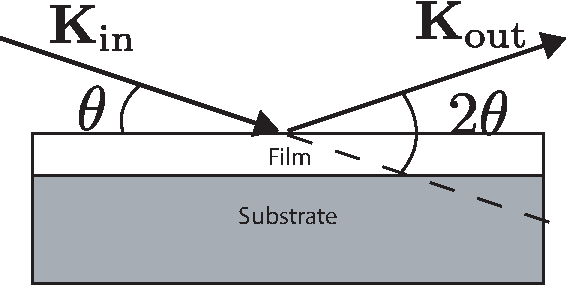
\includegraphics[width=.5\textwidth]{figures/techniques/xrr_schematic.pdf}
    \caption[X-ray reflectivity experimental schematic]{Schematic for x-ray reflectivity depicting the relevant geometry of the sample with respect to the incident ($\vec{K}_\mathrm{in}$) and scattered ($\vec{K}_\mathrm{out}$) radiation}
    \label{fig:xrr_schematic}
\end{figure}
Because the index of refraction $n$ for x-rays:
\begin{equation}
    n = 1 - \delta + i \beta
    \label{eq:x-ray_refractive}
\end{equation}
is smaller than unity, they undergo total external reflection at small incidence angles.  
As the incident angle is increased, a critical angle $\theta_c$ is reached and x-rays now enter the thin film material.  
Using Snell's law and Equation~\ref{eq:x-ray_refractive}, one can calculate the critical angle for x-rays $\theta_c = \sqrt{2 \delta}$ where $\delta \propto \rho$, the material's density~\cite{Als-Nielsen2011}.  
As the incident angle $\theta$ is further increased, the beam will travel through the film prior to reflecting from the film-substrate interface, picking up a phase difference with the beam that is reflected from the film-vacuum interface.  
This phase difference results in constructive and destructive interference, appearing as intensity oscillations with a period proportional to the film thickness.  

An experimentally measured XRR profile from a \SI{20}{\nm} LSMO film on NGO substrate is shown in Figure~\ref{fig:xrr_plot}.  
\begin{figure}[tb!]
    \centering
    \includegraphics[width=.65\textwidth]{figures/techniques/xrr.pdf}
    \caption[XRR data from a \SI{20}{\nm} LSMO film on NGO]{XRR data from a \SI{20}{\nm} LSMO film on NGO}
    \label{fig:xrr_plot}
\end{figure}
The intensity increase below \SI{0.6}{\degree} is an effect of the finite beam footprint and can be accounted for by using a simple footprint correction procedure using known values for the beam width and sample size.  
Figure~\ref{fig:xrr_plot} also shows a best fit to the experimental XRR curve, generated using the GenX program.  
GenX uses the Parratt formalism to simulate specular reflectivity curves that are then fit to experimental data using a genetic evolution algorithm~\cite{Bjorck2007}.  
Inputs into the fit include the film and substrate roughness and density, the film thickness, and specifics of the experimental geometry.  
Results from the fitting are given in Table~\ref{tab:xrr_techniques_results}
\begin{table}[tb!]
\centering
\caption{Structural parameters determined from the XRR fit in Figure~\ref{fig:xrr_plot}.  Absolute log figure of merit for this fit is \SI{0.0503}{}}
\label{tab:xrr_techniques_results}
\begin{tabular}{@{}p{2cm}p{2cm}p{2cm}p{2cm}@{}}
\toprule
Layer  & Density (\si{\g\per\cm}) & Roughness (\si{\nm}) & Thickness (\si{\nm}) \\
\midrule
LSMO   & 6.24              &   0.98           &  21.2 \\ 
NGO    &  7.595             &    0.5           & - \\
\bottomrule
\end{tabular}
\end{table}

\section{X-Ray Diffraction}

X-ray diffraction (XRD) is an x-ray-based structural characterization technique that provides information about the crystal structure of the material.  
A high resolution x-ray diffractometer is required for the analysis of thin film heterostructures because of the narrow substrate diffraction peaks and small angular separation between features of interest.  
The experimental setup is similar to that of an XRR measurement; however, XRD measurements are typically not performed at grazing incidence and the fixed $\theta-2\theta$ geometrical restriction is lifted and consequently the incident angle is referred to as $\alpha$, where $\alpha$ is defined relative to the diffracting planes and not the sample surface.  
The usage of a four-circle x-ray diffractometer, depicted in Figure~\ref{fig:four_circ}, allows for rotations about additional axis notated as $\phi$ and $\chi$.  
\begin{figure}[tb!]
    \centering
    \includegraphics[width=.6\textwidth]{figures/techniques/four_circle.pdf}
    \caption{Schematic of a four-circle x-ray diffractometer.  From~\cite{zotero-1883}.}
    \label{fig:four_circ}
\end{figure}

If we consider the incident wave vector to be $\vec{K}_\mathrm{in}$ and the scattered wave vector $\vec{K}_\mathrm{out}$, the Laue condition for diffraction states that
\begin{equation}
    \vec{K}_\mathrm{in} - \vec{K}_\mathrm{out} = \vec{G}
\end{equation}
where $\vec{G}$ is a reciprocal lattice vector and 
\begin{equation}
    |\vec{G}| = \frac{2 \pi}{d}
\end{equation}
with $d$ being the distance between atomic planes of the same family~\cite{Simon2013}.  
The Laue diffraction condition emphasizes the importance of reciprocal space when performing an XRD measurement.  
Positions of diffraction peaks in reciprocal space can be found by calculating the Fourier transform of the real space lattice, and XRD scans can be easily represented by arcs through reciprocal space.  
Figure~\ref{fig:recip_space_strained} illustrates a small region of reciprocal space for a thin film that is under tensile strain, compared with a relaxed film in Figure~\ref{fig:recip_space_strained_relaxed}.  
\begin{figure}
     \centering
     \begin{subfigure}[b]{0.49\textwidth}
         \centering
         \includegraphics[width=\textwidth]{figures/techniques/recip_space_strained.pdf}
         \caption{}
         \label{fig:recip_space_strained}
     \end{subfigure}
     \hfill
     \begin{subfigure}[b]{0.49\textwidth}
         \centering
         \includegraphics[width=\textwidth]{figures/techniques/recip_space_relaxed.pdf}
         \caption{}
         \label{fig:recip_space_strained_relaxed}
     \end{subfigure}
        \caption{Reciprocal space schematic for an (a) strained and (b) relaxed thin film that is under tensile strain.  Black dashed line depicts a symmetric $\omega-2\theta$ scan, blue dashed line is an asymmetric $\omega-2\theta$ scan through the \hkl(1 0 3) substrate peak, and the red box is a reciprocal space map about the \hkl(1 0 3) substrate peak}
        \label{fig:recip_space_schematic}
\end{figure}
Several types of scans through reciprocal space are indicated in Figure~\ref{fig:recip_space_schematic}.  
The black dashed line depicts a symmetric $\theta-2\theta$ scan, passing through peaks from both the film and substrate at different $2\theta$ values.  
A symmetric scan for crystal will have no in-plane component if the crystalline surface and lattice are aligned, therefore it will map out a line in reciprocal space that cuts through both film and substrate peaks irregardless of whether or not the film is relaxed.  
In contrast, an asymmetric scan is depicted by a blue dashed line in Figure~\ref{fig:recip_space_schematic} and will only lead to the diffraction condition being satisfied for the substrate peak in the strained film case.   
For both of these scans, Bragg's Law:
\begin{equation}
    \lambda = 2 d \sin \theta
    \label{eq:bragg_law}
\end{equation}
can be used to relate the diffracted peak's angular position $\theta$ to the crystalline lattice spacing $d$.  
A typical symmetric $\theta-2\theta$ XRD scan from an LSMO film on NGO substrate is shown in Figure~\ref{fig:xrd_simple}, taken around the substrate \hkl(2 2 0)$_\mathrm{o}$ = \hkl(0 0 2)$_{\mathrm{pc}}$ peak.  
\begin{figure}[tb!]
    \centering
    \includegraphics[width=.65\textwidth]{figures/techniques/xrd.pdf}
    \caption[$\omega-2\theta$ scan of \SI{20}{\nm} LSMO on NGO]{$\omega-2\theta$ scan of \SI{20}{\nm} LSMO on NGO showing the narrow substrate peak, a broad film peak, and Kiessig fringes.  Best fit simulated with xrayutilities shown in black.}
    \label{fig:xrd_simple}
\end{figure}
Peaks from both the substrate and LSMO film are readily observed and can be differentiated by comparing both the peak intensity and shape. 
The substrate is bulk-like leading to narrow and intense peaks.  
The diffraction peak for a thin layer is broad in the out of plane direction due to finite size effects~\cite{Cullity1956}.  
Presence of defects within the film can also lead to variations in the lattice parameter resulting in a broad peak.  
Oscillations on either side of the diffraction peaks are referred to as Kiessig fringes, indicative of smooth films with uniform d-spacing between layers throughout the film thickness.  
For thicker films the oscillation periodicity will be of a higher frequency.  

Another complimentary type of scan is a rocking curve, which is performed by fixing the detector angle $2\theta$ and ``rocking'' the incident angle $\alpha$.  
Rocking curves are sensitive to any misorientation in the material, also referred to as mosaicity.  
A rocking curve for an ideal material is very sharp, while higher mosaicity broadens the curve.  
Similar full width half maxima for the film and substrate peaks is a sign of a high quality film with similar structural quality as the substrate.  

The best fit to the radial $\theta-2\theta$ data set, shown as a black line in Figure~\ref{fig:xrd_simple}, was generated with xrayutilities~\cite{Kriegner2013b}, a collection of python scripts for reduction, simulation, and fitting of x-ray diffraction data.  
A dynamical diffraction model was used to simulate the diffraction profile and a differential evolution algorithm was used to fit the experimental dataset.  
Inputs to the model include the film thickness and out-of-plane lattice parameter.  
From this fit, the thickness was determined to be \SI{20.1}{\nm} with a c/a ratio of 1.016, where the in-plane lattice parameter (a) was assumed to be an average of the two in-plane distances for \hkl(1 1 0)$_\mathrm{o}$-oriented NGO substrates.  

The last type of reciprocal space scan used in this work is a reciprocal space map (RSM), denoted by the red shaded area in Figure~\ref{fig:recip_space_schematic}.  
By combining a number of different line scans a small area of reciprocal space is analyzed.  
An RSM is especially useful for analyzing the strain state of a thin film because unlike the asymmetric line scans, an RSM will map out a large area of reciprocal space containing both the film peak and substrate peak for both the strained and relaxed cases.  
Figure~\ref{fig:rsm} shows an RSM about the \hkl(1 0 3)$_\mathrm{pc}$ peak for a \SI{6}{\nm} LSMO / \SI{12}{\nm} LSCO bilayer on a \hkl(1 1 0)$_\mathrm{o}$-oriented NGO substrate.  
\begin{figure}[tb!]
    \centering
    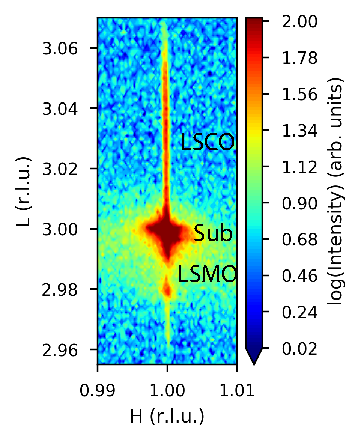
\includegraphics[width=.5\textwidth]{figures/techniques/na08_103_rsm.pdf}
    \caption{RSM about the NGO (103)$_\mathrm{pc}$ peak for a \SI{6}{\nm} LSMO / \SI{12}{\nm} LSCO bilayer.}
    \label{fig:rsm}
\end{figure}
The vertical alignment of the LSMO and LSCO peaks with the substrate peak indicate that they are coherently strained with the substrate.  

\section{Vibrating Sample Magnetometry}

A vibrating sample magnetometer (VSM) was used to study magnetic switching behavior of the complex oxide thin films.  
In a VSM a sample is mounted on a nonmagnetic rod, placed within a cryogenic chamber, and driven at a high frequency between a set of pickup coils.  
If the sample is magnetized, its motion through the pickup coils produces a small oscillatory emf, proportional to the sample magnetization~\cite{Cullity2011}.  
The entire VSM assembly is placed within a cryostat within a superconducting solenoid able of producing magnetic fields with sufficient strength to magnetically switch all layers in a heterostructure.  
In this way, the VSM is able to measure the net magnetic moment of a sample as a function of temperature or changing magnetic field.  

\section{X-Ray Spectroscopy}
X-ray absorption (XA) spectroscopy is a powerful characterization technique used to obtain information about the valence state and bonding configuration of individual ions within a material.  
In XAS, incident x-rays are tuned to a specific electronic transition, in this case the L-edge energy for either \ce{Co} or \ce{Mn} corresponding to electronic transitions from filled 2p to empty 3d levels.  
A schematic for this transition is shown in Figure~\ref{fig:xas_levels}.   
\begin{figure}[b!]
    \centering
    \includegraphics[width=.3\textwidth]{figures/techniques/l-edge_xas.png}
    \caption[L-edge x-ray absorption spectroscopy electronic transitions]{L-edge x-ray absorption spectroscopy electronic transitions.  Incident x-rays with an energy $h\nu$ excite electrons from filled p to empty d-levels.  The 2p$_{1/2}$-3d transition is called the L$_2$ edge and the 2p$_{3/2}$-3d transition is the L$_3$ edge}
    \label{fig:xas_levels}
\end{figure}
Because the 2p level is split into 2p$_{1/2}$ and 2p$_{3/2}$ energy levels due to spin-orbit coupling, two absorption peaks corresponding to the 3d transitions are observed, with the L$_3$ peak at lower energies and the L$_2$ peak at higher energies.  
XA spectra are highly sensitive to both the ion valence and local bonding environment: Figure~\ref{fig:simple_xas} depicts Co L-edge spectra for three different materials, LSCO with a mixture of \ce{Co^3+} and \ce{Co^4+} ions, \ce{LaCoO3} with \ce{Co^3+} ions, and \ce{La2CoMnO6} with \ce{Co^2+} ions.  
\begin{figure}[tb]
    \centering
    \includegraphics[width=.65\textwidth]{figures/techniques/xas_xmcd_example.pdf}
    \caption{XA and XMCD spectra for LSCO, \ce{LaCoO3}, and \ce{La2CoMnO6} highlighting the spectral changes for different Co valence.}
    \label{fig:simple_xas}
\end{figure}
\ce{LSCO} shows a symmetric L$_2$ peak compared with \ce{LaCoO3}, while the L$_3$ peak for LSCO shifts to higher energies signifying the presence of a mixed \ce{Co^3+}/\ce{Co^4+} valence state~\cite{Merz2010}.  
In contrast, \ce{La2CoMnO6} has an L$_3$ peak at lower energies than both \ce{LaCoO3} and LSCO while also showing a complex multiplet structure at the L$_3$ edge.  
As the Co valence changes, the filling of the 3d orbitals also changes, leading to the observed differences in XA spectra.  

There are a number of different ways in which the XA signal can be measured, including total electron yield (TEY) detection and luminescence yield (LY) detection.  
When an x-ray is absorbed by an atom, a core level electron is emitted from the 2p level and the process of filling this core hole generates a cascade of secondary and Auger electrons.  
By monitoring the current required to maintain sample neutrality,  a sample's x-ray absorption can be measured.  
Electrons have a finite mean free path meaning that XA spectra in TEY mode do not provide information from the entire volume of material.  
For oxides, the mean free path is approximately \SI{5}{\nm} - \SI{10}{\nm}~\cite{Shibata2014}.  
In contrast to TEY detection, LY detection gives information averaged over the sample depth.  
LY signal arises in a luminescent substrate that converts incident x-ray photons into visible light photons - if x-rays are absorbed by the film material they will not reach the substrate so the signal will be reduced~\cite{Bianconi1978}.  
Raw LY data is then converted to XA by taking the negative log of the dataset~\cite{vanderLaan2014}.  

X-ray Magnetic Circular Dichroism (XMCD) provides element specific magnetic information.  
By using circularly polarized light, electrons can be excited from 2p levels with a preferred spin direction: right circularly polarized light excites \SI{62.5}{\percent} spin up electrons from the 2p$_{3/2}$ level and \SI{75}{\percent} spin down electrons from the 2p$_{1/2}$ level~\cite{vanderLaan2014}.  
Different spins are preferentially excited to the valence level from the spin-orbit split 2p$_{1/2}$ and 2p$_{3/2}$ levels because the spin orbit coupling is opposite.  
In a ferromagnet, the exchange interaction results in the density of states for opposing spin directions being shifted with respect to one another.  
Because of this shift, there is a difference in the available states for spin up and spin down electrons near the Fermi level and therefore the absorption of right and left circularly polarized light, which depends upon the number of empty states, is not equal.  
An XMCD spectra is taken as the difference in absorption for the two circular polarization directions, with the signal being proportional to the orientation of the sample magnetization vector with respect to the x-ray helicity as well as the amount of circular polarization in the incident x-ray beam.  
Figure~\ref{fig:vanderlaan_xmcd} outlines the XMCD process.  
\begin{figure}[tb]
    \centering
    \includegraphics[width=.3\textwidth]{figures/techniques/xmcd_vanderlaan.png}
    \caption[XMCD absorption process]{XMCD absorption process.  Right circularly polarized light ($\mu^+$) and left circularly polarized light ($\mu^-$) preferentially excite electrons of different spin directions.  Because there is an imbalance of holes of opposite spin directions the absorption process is dependent on the direction of circular polarization.  From~\cite{vanderLaan2014}}
    \label{fig:vanderlaan_xmcd}
\end{figure}
An external magnetic field H is applied to the sample to align all magnetic domains to point in the same direction.  
The XMCD signal can also be acquired with a constant circular polarization by collecting energy scans with the field pointing in opposite directions and taking the difference.  
Experimentally measured XMCD spectra are presented in the bottom panel of Figure~\ref{fig:simple_xas}.  
Again, distinct differences occur with different Co valence with the most dramatic change being the shape of the \ce{La2CoMnO6} \ce{Co^2+} spectra compared with the LSCO and \ce{LaCoO3} spectra.  
Along with XMCD energy scans outlined above, XMCD can also be used to gather element specific magnetic hysteresis loops by tracking the XMCD signal as a function of applied field strength with the incident photon energy fixed to the maximum XMCD signal.  

Both XA and XMCD spectra are invaluable characterization techniques, providing information about the valence state, bonding configurations, and magnetic state of individual layers in a complex oxide heterostructure.  
Most importantly both of these techniques used are element-specific providing a way to extract information from individual layers in a complex oxide heterostructure.  

\section{Conclusion}
By controlling the parameters for PLD growth, high quality complex oxide heterostructures are synthesized.  
Structural characterization using XRR and XRD confirms the film thickness, crystalline quality, and also provides relevant information about the crystallographic relationship between layers in a heterostructure.  
Finally, by utilizing XA and XMCD spectroscopy along with VSM magnetometry a complete picture of the electronic and magnetic landscape is acquired.  

    %!TEX root = ../main.tex
\chapter{Structural Characterization of LSMO / LSCO Bilayers}
This chapter discusses structural characterization of \ce{La_{0.7}Sr_{0.3}MnO3} (LSMO) and \ce{La_{0.7}Sr_{0.3}CoO3} (LSCO) single layer films and bilayers.  
Basic structural characterization using x-ray reflectivity (XRR) and x-ray diffraction (XRD) in order to characterize the film thickness, strain state, and out-of-plane lattice parameter are first discussed, followed by analysis of half-order diffraction peaks to determine octahedral rotation patterns.  
Simulations of half-order diffraction peaks to quantitatively determine octahedral rotation angles are also discussed.  

\section{Experimental Methods}
A series of single layer LSCO and LSMO films as well as LSMO / LSCO bilayers were grown on \hkl(1 1 0)$_o$-oriented \ce{NdGaO3} (NGO) substrates via pulsed laser deposition (PLD).  
Laser energy density was set to \SI{1}{\joule\per\cm\squared} at a repetition rate of \SI{1}{\hertz} under a \ce{O2} pressure of \SI{300}{\milli\torr} while the substrate was held at \SI{700}{\celsius}.  
Following deposition, the films were slowly cooled to room temperature in \ce{O2} environment (\SI{300}{\torr}).  
The naming convention for single layer LSCO and LSMO films is (C, M)x where the C or M denotes LSCO or LSMO respectively and x is the layer thickness in \si{nm}.  
For LSMO / LSCO bilayers a CxMy naming convention is used, where x is the LSCO layer thickness and y is the LSMO layer thickness in \si{nm}.  

XRR measurements were performed on a Bruker D8 Discover four circle diffractometer equipped with a Goebel mirror to isolate the \ce{Cu} K$\alpha$ radiation.  
Diffraction experiments were performed on the same experimental setup with an additional \ce{Ge} \hkl(2 2 0) two-bounce monochromator producing monochromatic \ce{Cu} K$\alpha_1$ radiation.  
Radial $\theta-2\theta$ scans were measured about the NGO \hkl(2 2 0)$_o$ peak.  
Reciprocal space maps (RSMs) were measured around the NGO \hkl(4 2 0)$_o$ and \hkl(3 3 2)$_o$ peaks.  
Synchrotron-based diffraction measurements were performed at beamline 7-2 of the Stanford Synchrotron Radiation Lightsource with an x-ray energy of \SI{14}{\kilo\eV}.  
All structural characterization measurements were performed at room temperature.  

\section{X-Ray Reflectivity}
The XRR profiles for single layer LSCO films C12, C8, C4, C2, as well as single layer LSMO film M6, are plotted in Figure~\ref{fig:singlelayer_xrr}.  
\begin{figure}[b!]
    \centering
    \includegraphics[width=.6\textwidth]{figures/results1/single_xrr.pdf}
    \caption{XRR profiles for LSCO single layer films C12, C8, C4, and C2, and LSMO single layer M6.  Best fits to the experimental datasets were generated with GenX and are shown as black lines using a single layer film model.}
    \label{fig:singlelayer_xrr}
\end{figure}
All films except for single layer C2 show Kiessig fringes, indicative of high quality films with smooth interfaces.  
A combination of low sample thickness and limited signal-to-noise ratio of the lab-based setup is responsible for the lack of observable fringes for sample C2.  
Best fits to the experimental XRR profiles were generated with GenX using a single layer film model with a carbon cap to account for potential surface contamination and are depicted as black lines in Figure~\ref{fig:singlelayer_xrr}.  
Inputs to the XRR model include the thickness ($t$), roughness ($\sigma$), and density ($\rho$) of the film and substrate.  
The substrate and film roughness, film thickness, and film density are all allowed to vary in the fits while the substrate density is fixed to its bulk value.  
An absolute logarithmic difference was used as a figure of merit to compare the goodness of fit.  
Structural parameters derived from the GenX fitting results for single layer films are outlined in Tables~\ref{tab:c12_xrr}-\ref{tab:cm6_xrr}.  
When fitting XRR curves with GenX, the error in a fit parameter can be calculated by letting that parameter freely vary over a range of values and selecting the error bounds to correspond with a $\pm 5\%$ increase around the optimal figure of merit.  
Error on thickness values calculated with this method for the single layer GenX fits are within $\pm \SI{2}{\angstrom}$ of the given thickness value.  
%%%%%%%%%%%%%%%%%%
%%%%%%C12%%%%%%%
%%%%%%%%%%%%%%%%%%
\begin{table}[tb!]
\centering
\caption{Results from GenX fits for sample C12. FOM = \SI{3.79e-2}{}}
\label{tab:c12_xrr}
\begin{tabular}{@{}llll@{}}
\toprule
Layer & $t$ (\si{nm}) & $\sigma$ (\si{nm}) & $\rho$ (\si{\gram\per\cm\cubed})\\ \midrule
Carbon cap & 0.81 & 0.118 & 2.25 \\
LSCO & 11.32 & 0.532 & 6.77\\
NGO & N/A & 0.489 & 7.59\\
\bottomrule
\end{tabular}
\end{table}
%%%%%%%%%%%%%%%%%%
%%%%%%C8%%%%%%%
%%%%%%%%%%%%%%%%%%
\begin{table}[tb!]
\centering
\caption{Results from GenX fits for sample C8. FOM = \SI{4.17e-2}{}}
\label{tab:c8_xrr}
\begin{tabular}{@{}llll@{}}
\toprule
Layer & $t$ (\si{nm}) & $\sigma$ (\si{nm}) & $\rho$ (\si{\gram\per\cm\cubed})\\ \midrule
Carbon cap & 0.78 & 0.423 & 2.24 \\
LSCO & 7.86 & 0.401 & 6.76\\
NGO & N/A & 0.271 & 7.59\\
\bottomrule
\end{tabular}
\end{table}
%%%%%%%%%%%%%%%%%%
%%%%%%C4%%%%%%%
%%%%%%%%%%%%%%%%%%
\begin{table}[tb!]
\centering
\caption{Results from GenX fits for sample C4. FOM = \SI{6.19e-2}{}}
\label{tab:c4_xrr}
\begin{tabular}{@{}llll@{}}
\toprule
Layer & $t$ (\si{nm}) & $\sigma$ (\si{nm}) & $\rho$ (\si{\gram\per\cm\cubed})\\ \midrule
Carbon cap & 0.95 & 0.426 & 2.23 \\
LSCO & 3.80 & 0.310 & 6.66\\
NGO & N/A & 0.271 & 7.59\\
\bottomrule
\end{tabular}
\end{table}
%%%%%%%%%%%%%%%%%%
%%%%%%C2%%%%%%%
%%%%%%%%%%%%%%%%%%
\begin{table}[tb!]
\centering
\caption{Results from GenX fits for sample C2. FOM = \SI{3.01e-2}{}}
\label{tab:c2_xrr}
\begin{tabular}{@{}llll@{}}
\toprule
Layer & $t$ (\si{nm}) & $\sigma$ (\si{nm}) & $\rho$ (\si{\gram\per\cm\cubed})\\ \midrule
Carbon cap & 0.65 & 0.489 & 1.72 \\
LSCO & 1.51 & 0.263 & 5.43\\
NGO & N/A & 0.735 & 7.59\\
\bottomrule
\end{tabular}
\end{table}
%%%%%%%%%%%%%%%%%%
%%%%%%M6%%%%%%%
%%%%%%%%%%%%%%%%%%
\begin{table}[tb!]
\centering
\caption{Results from GenX fits for sample M6. FOM = \SI{2.42e-2}{}}
\label{tab:cm6_xrr}
\begin{tabular}{@{}llll@{}}
\toprule
Layer & $t$ (\si{nm}) & $\sigma$ (\si{nm}) & $\rho$ (\si{\gram\per\cm\cubed})\\ \midrule
Carbon cap & 1.14 & 0.678 & 2.21 \\
LSMO & 6.37 & 0.359 & 6.32\\
NGO & N/A & 0.474 & 7.59\\
\bottomrule
\end{tabular}
\end{table}

There is good agreement between experimental data and simulated fits for all of the single layer films except for sample C4 which has a poor fit to the thickness fringe periodicity and a larger figure of merit compared with other fits.  
The poor fit for sample C4 results in a higher uncertainty on the film thickness and density compared with the other single layer films.  
Ignoring single layer C2 that shows no obvious features to fit, as well as sample C4 with a poor fit, the experimentally determined film thickness is within \SI{10}{\percent} of the desired film thickness for all of the single layer films and they all have a roughness below \SI{1}{\nm} indicating high quality films.  
In addition, densities extracted from the fits are within several percent of the bulk values of \SI{6.788}{\g\per\cm\cubed} for LSCO and \SI{6.427}{\g\per\cm\cubed} for LSMO indicating a low number of defects such as oxygen vacancies.   

XRR profiles from bilayers C12M6, C8M6, C4M6, and C2M6, along with their GenX fits, are presented in Figure~\ref{fig:bilayer_xrr}.  
\begin{figure}[tb]
    \centering
    \includegraphics[width=.6\textwidth]{figures/results1/bilayer_xrr.pdf}
    \caption{XRR profiles for LSMO / LSCO bilayers C12M6, C8M6, C4M6, and C2M6.  Best fits to the experimental datasets were generated with GenX and are shown as black lines.}
    \label{fig:bilayer_xrr}
\end{figure}
A three layer model was used to fit the bilayer samples with one LSCO layer, one  LSMO layer, and a carbon cap to account for surface contamination.  
Structural parameters derived from the GenX fits to bilayer LSMO / LSCO are given in Tables~\ref{tab:c12m6_xrr}-\ref{tab:c2m6_xrr}.  
The uncertainty on the thickness values for the bilayer fits is within \SI{2}{\angstrom}, calculated in a similar way as with the single layer fits.  
Although individual LSCO and LSMO layer thicknesses are quoted in the bilayer XRR fitting results, only the total layer thickness is accurate.  
XRR is sensitive to differences in atomic scattering factors between individual layers, and because LSMO and LSCO have similar atomic scattering factors at the non-resonant \ce{Cu} K$\alpha$ energy, XRR does not differentiate well between the two materials.  
%%%%%%%%%%%%%%%%%%
%%%%%%C12M6%%%%%%%
%%%%%%%%%%%%%%%%%%
\begin{table}[tb!]
\centering
\caption{Results from GenX fits for bilayer C12M6. FOM = \SI{2.41e-2}{}}
\label{tab:c12m6_xrr}
\begin{tabular}{@{}llll@{}}
\toprule
Layer & $t$ (\si{nm}) & $\sigma$ (\si{nm}) & $\rho$ (\si{\gram\per\cm\cubed})\\ \midrule
Carbon cap & 1.18 & 0.803 & 1.95 \\
LSMO & 5.89 & 0.312 & 6.46\\
LSCO & 11.14 & 0.327 & 6.64\\
NGO & N/A & 0.377 & 7.59\\
\bottomrule
\end{tabular}
\end{table}
%%%%%%%%%%%%%%%%%%
%%%%%%C8M6%%%%%%%
%%%%%%%%%%%%%%%%%%
\begin{table}[tb!]
\centering
\caption{Results from GenX fits for bilayer C8M6. FOM = \SI{3.02e-2}{}}
\label{tab:c8m6_xrr}
\begin{tabular}{@{}llll@{}}
\toprule
Layer & $t$ (\si{nm}) & $\sigma$ (\si{nm}) & $\rho$ (\si{\gram\per\cm\cubed})\\ \midrule
Carbon cap & 1.34 & 0.691 & 2.06 \\
LSMO & 5.63 & 0.265 & 6.28\\
LSCO & 8.41 & 0.352 & 6.54\\
NGO & N/A & 0.353 & 7.59\\
\bottomrule
\end{tabular}
\end{table}
%%%%%%%%%%%%%%%%%%
%%%%%%C4M6%%%%%%%
%%%%%%%%%%%%%%%%%%
\begin{table}[tb!]
\centering
\caption{Results from GenX fits for bilayer C4M6. FOM = \SI{3.68e-2}{}}
\label{tab:c4m6_xrr}
\begin{tabular}{@{}llll@{}}
\toprule
Layer & $t$ (\si{nm}) & $\sigma$ (\si{nm}) & $\rho$ (\si{\gram\per\cm\cubed})\\ \midrule
Carbon cap & 0.940 & 0.480 & 2.24 \\
LSMO & 5.62 & 0.252 & 6.37\\
LSCO & 4.01 & 0.481 & 6.62\\
NGO & N/A & 0.366 & 7.59\\
\bottomrule
\end{tabular}
\end{table}
%%%%%%%%%%%%%%%%%%
%%%%%%C2M6%%%%%%%
%%%%%%%%%%%%%%%%%%
\begin{table}[tb!]
\centering
\caption{Results from GenX fits for bilayer C2M6. FOM = \SI{3.03e-2}{}}
\label{tab:c2m6_xrr}
\begin{tabular}{@{}llll@{}}
\toprule
Layer & $t$ (\si{nm}) & $\sigma$ (\si{nm}) & $\rho$ (\si{\gram\per\cm\cubed})\\ \midrule
Carbon cap & 1.80 & 0.925 & 1.84 \\
LSMO & 5.05 & 0.412 & 6.58\\
LSCO & 2.31 & 0.178 & 6.51\\
NGO & N/A & 0.348 & 7.59\\
\bottomrule
\end{tabular}
\end{table}
The XRR fits indicate high quality films with low layer roughness, with thicknesses close to the target values.  

\section{X-Ray Diffraction}
$\theta-2\theta$ scans were performed about the NGO \hkl(2 2 0)$_o$ peak.  
NGO is an orthorhombic substrate with $a=\SI{5.43}{\angstrom}$, $b=\SI{5.50}{\angstrom}$, and $c=\SI{7.71}{\angstrom}$.  
A pseudocubic (pc) unit cell can be constructed with a \hkl(1 1 0)$_o$ $||$ \hkl(0 0 1)$_{pc}$ and \hkl(0 0 2)$_o$ $||$ \hkl(1 0 0)$_{pc}$ transformation, resulting in $a_{pc}=\SI{3.855}{\angstrom}$, $b_{pc}=\SI{3.864}{\angstrom}$, and $c_{pc}=\SI{3.864}{\angstrom}$.  
With this pseudocubic transformation, the NGO \hkl(2 2 0)$_o$ peak corresponds with a \hkl(0 0 2)$_{pc}$ peak.  

The pseudocubic lattice parameter for LSCO is \SI{3.844}{\angstrom} while that of LSMO is \SI{3.873}{\angstrom}.  
Therefore, when LSMO and LSCO are grown on \hkl(1 1 0)$_o$ NGO substrates, LSCO will be under tensile strain with a lattice mismatch of \SI{.402}{\percent} while LSMO will be under compressive strain with a lattice mismatch of \SI{-.350}{\percent}.  
$\theta-2\theta$ scans through the \hkl(2 2 0)$_o$ peak should show a film peak on the high angle side of the substrate for LSCO films and on the low angle side for LSMO films.  
$\theta-2\theta$ scans around the NGO \hkl(2 2 0)$_o$ for single layer films are shown in Figure~\ref{fig:singlelayer_xrd} and for bilayer films in Figure~\ref{fig:bilayer_xrd}.  
The film peaks in the $\theta-2\theta$ scans are at their expected locations on either side of the substrate peak.  
\begin{figure}[tb!]
    \centering
    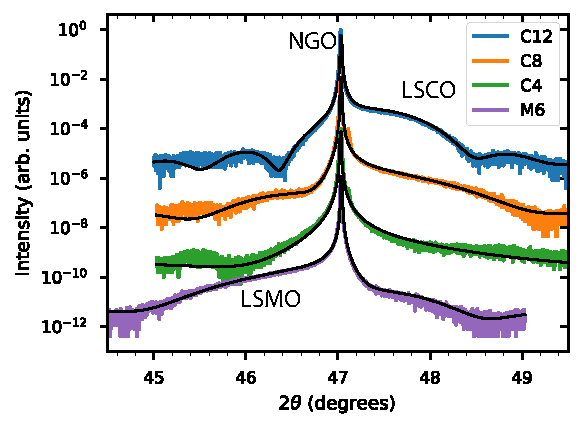
\includegraphics[width=.6\textwidth]{figures/results1/single_220.pdf}
    \caption{$\theta-2\theta$ scan about the NGO \hkl(2 2 0)$_o$ peak for single layer films C12, C8, C4, and M6}
    \label{fig:singlelayer_xrd}
\end{figure}
\begin{figure}[tb!]
    \centering
    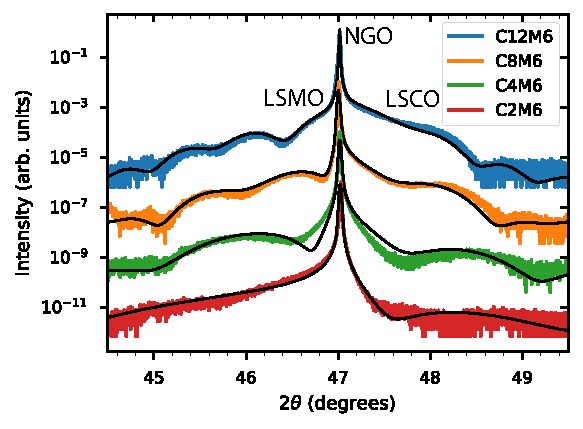
\includegraphics[width=.6\textwidth]{figures/results1/bilayer_220.pdf}
    \caption{$\theta-2\theta$ scan about the NGO \hkl(2 2 0)$_o$ peak for bilayer films C12M6, C8M6, C4M6, and C2M6}
    \label{fig:bilayer_xrd}
\end{figure}
\begin{table}[b!]
\centering
\caption{Structural parameters from xrayutilities fits to single layers C12, C8, C4, and M6. 3$\sigma$ confidence intervals reported in parenthesis.}
\label{tab:singlelayer_xrd}
\begin{tabular}{@{}lll@{}}
\toprule
Sample & $t$ (\si{nm}) & $c$ (\si{\angstrom}) \\ \midrule
C12 & 11.20(23) & 3.819(2) \\
C8 & 6.15(29) & 3.814(3) \\
C4 & 2.31(25) & 3.832(7) \\
M6 & 6.17(20) & 3.924(3)  \\
\bottomrule
\end{tabular}
\end{table}
\begin{table}[tb!]
\centering
\caption{Structural parameters from xrayutilities fits to LSMO / LSCO bilayers. 3$\sigma$ confidence intervals reported in parenthesis.}
\label{tab:bilayer_xrd}
\begin{tabular}{@{}lllllll@{}}
\toprule
& & \multicolumn{2}{c}{LSCO} & & \multicolumn{2}{c}{LSMO} \\
\cmidrule{3-4} \cmidrule{6-7}
Sample && $t$ (\si{nm}) & $c$ (\si{\angstrom}) && $t$ (\si{nm}) & c (\si{\angstrom})\\ \midrule
C12M6 && 9.94(25) & 3.815(2) && 5.29(18) & 3.908(4)\\
C8M6 && 6.18(26) & 3.801(3) && 6.21(14) & 3.909(3) \\
C4M6 && 3.30(43) & 3.840(1) && 5.01(11) & 3.902(1) \\
C2M6 && 0.50(13) & 3.813(32) && 4.51(6) & 3.924(2) \\
\bottomrule
\end{tabular}
\end{table}
Fits generated using a dynamical diffraction model, created with xrayutilities~\cite{Kriegner2013b}, are overlaid on the experimental data as black lines.  
For the fits, the NGO out-of-plane lattice parameter was fixed to \SI{3.864}{\angstrom} while the film thicknesses and lattice parameters were allowed to freely vary.  
The model used for XRD fits consists of a single layer for each material with a constant out-of-plane lattice parameter.  
A peak at \SI{45.5}{\degree} arises due to tungsten contamination of the copper x-ray tube, and is not captured by the XRD fits.  
Structural parameters derived from the single layer fits are given in Table~\ref{tab:singlelayer_xrd} while those from bilayer fits are in Table~\ref{tab:bilayer_xrd}.  
The reported errors correspond with a $3-\sigma$ confidence interval, with the typical error being within \SI{.003}{\angstrom} for the lattice parameter and \SI{.25}{\nm} for the layer thickness.  
For the single layer films, the LSCO lattice parameter is not sensitive to variation in LSCO film thickness.  
C4 has a slightly larger out-of-plane lattice parameter; however, the absence of any prominent features in the $\theta-2\theta$ scan for C4 suggests the out-of-plane lattice parameter derived from fits is not reliable.  
Poor fits to the diffuse scattering around the substrate peak for bilayer C4M6 also indicate that the model used is not completely accurate.  

$\theta-2\theta$ scans were also measured for samples C12, M6, and C12M6 at a SSRL beamline 7-2.  
Experimental data with fits are shown in Figure~\ref{fig:ssrl_xrd}, with structural parameters from the fits in Table~\ref{tab:ssrl_xrd}.  
The diffraction peak shapes are fit well for all samples, while thickness oscillations for sample C12M6 are not well fit on the high angle side of the main diffraction peak.  
\begin{figure}[tb]
    \centering
    \includegraphics[width=.6\textwidth]{figures/results1/ssrl_fits.pdf}
    \caption{$\theta-2\theta$ scans and fits for C12M6, C12, and M6, measured at SSRL BL 7-2}
    \label{fig:ssrl_xrd}
\end{figure}
\begin{table}[tb!]
\centering
\caption{Structural parameters from xrayutilities fits to BL 7-2 $\theta-2\theta$ scans.  3$\sigma$ confidence intervals reported in parenthesis.}
\label{tab:ssrl_xrd}
\begin{tabular}{@{}lllllll@{}}
\toprule
& & \multicolumn{2}{c}{LSCO} & & \multicolumn{2}{c}{LSMO} \\
\cmidrule{3-4} \cmidrule{6-7}
Sample && $t$ (\si{nm}) & $c$ (\si{\angstrom}) && $t$ (\si{nm}) & c (\si{\angstrom})\\ \midrule
C12M6 && 10.37(20) & 3.809(3) && 5.37(13) & 3.912(4)\\
C12 && 11.30(15) & 3.819(3) && - & - \\
M6 && - & - && 5.97(12) & 3.931(4) \\
\bottomrule
\end{tabular}
\end{table}
The higher dynamic range of synchrotron-based measurements results in the observation of significantly more thickness fringes compared with a lab-source and therefore the thickness values in Table~\ref{tab:ssrl_xrd} are considered to be more accurate compared with values derived from the lab-based diffractometer.  
Considering the uncertaity, the derived thicknesses and lattice parameters from both the synchrotron and lab-based diffractometer are in close agreement.  

There is a slight discrepancy between total film thicknesses derived from XRR fits and those from XRD fits, especially for the bilayer sample series.  
The total thickness for bilayers C12M6, C8M6, and C4M6 from lab-based XRD fits is \SI{10}{\percent} smaller than from XRR fits, and for bilayer C2M6 the difference is even more pronounced with a \SI{30}{\percent} difference between XRR and XRD derived thicknesses.  
When XRD data is fit, information about film thickness is derived by the diffracted peak shape.  
Thin films create broad diffraction peaks with low integrated peak intensity while thick films produce narrow peaks with high integrated peak intensity~\cite{Cullity1956}.  
Additional sources of peak broadening include the presence of any d-spacing variations within the film which can be caused by stoichiometry variations or relaxation.  
If d-spacing variations are present, a single layer model will account for additional broadness by altering the film thickness.  
Furthermore, XRD fits cannot account for the presence of any amorphous layers.  
Because XRR is insensitive to crystallographic information such as d-spacing variations or whether or not the film is crystalline or amorphous, there can be disagreement in XRR and XRD derived film thicknesses.  

\section{Reciprocal Space Maps}

Reciprocal space maps (RSM) were recorded about the NGO \hkl(3 3 2)$_o$ = \hkl(1 0 3)$_{pc}$ and \hkl(4 2 0)$_o$ = \hkl(0 1 3)$_{pc}$ peaks, which are rotated by \SI{90}{\degree} in $\phi$ from one another.  
Maps must be recorded at both orientations to confirm films are coherently strained along the two inequivalent in-plane directions of the orthorhombic NGO substrate.  
Because NGO substrates are orthorhombic, the out-of-plane position of the \hkl(1 0 3)$_{pc}$ and \hkl(0 1  3)$_{pc}$ peaks will be at different locations in reciprocal space~\cite{Vailionis2011}.  
RSMs for single layer C12 are shown in Figure~\ref{fig:c12_asym_rsm}.  
The film and substrate peaks occur at the same in-plane value indicating that the film is coherently strained to the substrate.  
\begin{figure}[b!]
    \centering
    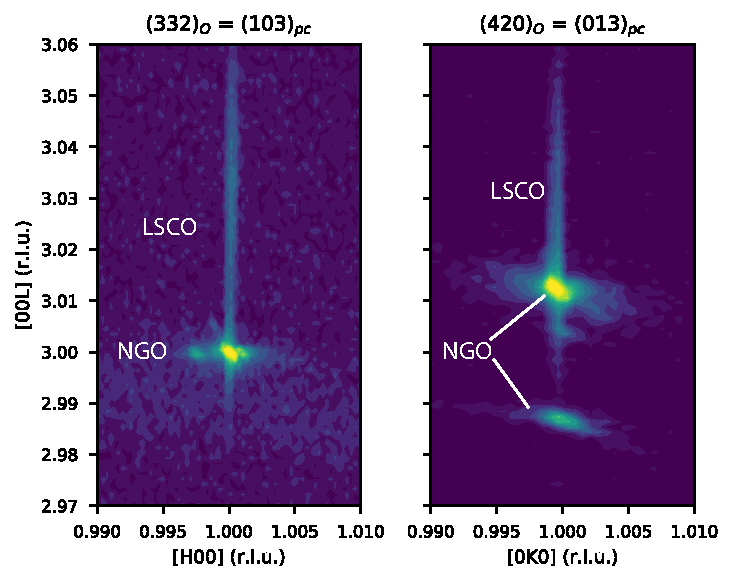
\includegraphics[width=.7\textwidth]{figures/results1/NA04_asym_rsms.pdf}
    \caption{C12 RSMs}
    \label{fig:c12_asym_rsm}
\end{figure}
RSMs for single layer C8 (Figure~\ref{fig:c8 rsm}), bilayer C12M6 (Figure~\ref{fig:c12m6_asym_rsm}), and bilayer C8M6 (Figure~\ref{fig:c8m6_rsm}) also confirm that these films are coherently strained.  
\begin{figure}[h!]
    \centering
    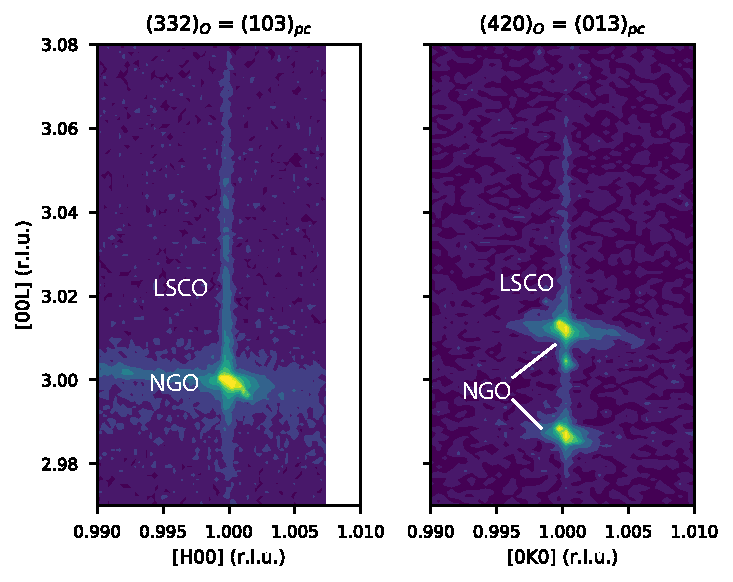
\includegraphics[width=.7\textwidth]{figures/results1/NA06_asym_rsms.pdf}
    \caption{C8 RSMs}
    \label{fig:c8 rsm}
\end{figure}
\begin{figure}[h!]
    \centering
    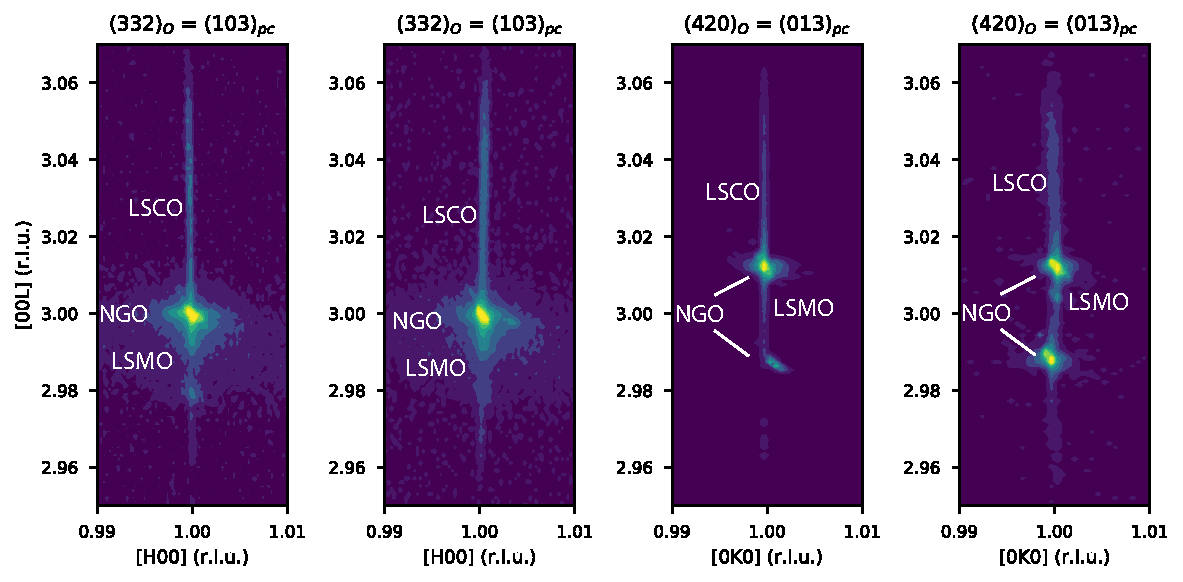
\includegraphics[width=\textwidth]{figures/results1/NA08_asym_rsms.pdf}
    \caption{C12M6 RSMs}
    \label{fig:c12m6_asym_rsm}
\end{figure}
\begin{figure}[h!]
    \centering
    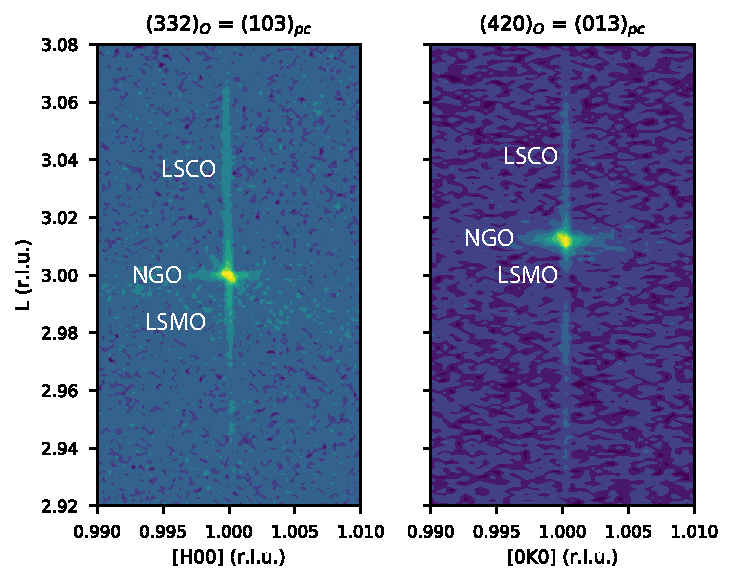
\includegraphics[width=.7\textwidth]{figures/results1/na09_asym_rsms.pdf}
    \caption{C8M6 RSMs}
    \label{fig:c8m6_rsm}
\end{figure}
The \hkl(4 2 0)$_o$ RSM shows two substrate peaks at different L positions for films C12, C8, and C12M6, while bilayer C8M6 only shows one substrate peak.  
This double substrate peak points to there being two structural domains within the substrate rotated \SI{180}{\degree} from one another.  
Substrate pieces are cut from a larger wafer, therefore certain substrate pieces may bisect both domains while others will only contain a single structural domain.  
RSMs about the \hkl(4 2 0)$_o$ peak are sensitive to the difference in the orthorhombic $a_o$ and $b_o$ directions and therefore the presence of rotated structural domains is only observable for this peak.  

A small tilt of approximately \SI{0.3}{\degree} between the LSCO film and substrate peak locations is present in the \hkl(3 3 2)$_o$ RSMs indicating that the film has bond angle deviation away from \SI{90}{\degree} along this direction.  
In Figure~\ref{fig:rsm_bond_angle}, a zoomed in image of the C12 \hkl(3 3 2)$_o$ RSM is shown making the bond angle deviation more clear. 
\begin{figure}[tb!]
    \centering
    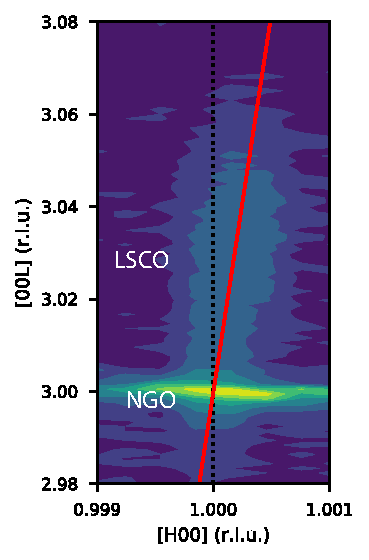
\includegraphics[width=.4\textwidth]{figures/results1/rsm_angle.pdf}
    \caption{C12 \hkl(3 3 2)$_{o}$ RSM zoomed in to emphasize the bond angle deviation from \SI{90}{\degree}}
    \label{fig:rsm_bond_angle}
\end{figure}
This deviation is only observed for \hkl(3 3 2)$_o$ RSMs meaning that this angle variation is only occurring for one of the bond angles resulting in a monoclinic unit cell for the growing LSCO and LSMO films on NGO substrates.  
The observed bond angle deviation has been reported for other perovskite films on orthorhombic substrates, such as \ce{SrRuO3} films on \ce{DyScO3} substrates~\cite{Vailionis2011}.   


\clearpage
\section{Diffraction from Half Order Peaks}
In the ideal perovskite structure, the B-O-B bond chains connecting each \ce{BO6} octahedra all make \SI{180}{\degree} angles leading to cubic symmetry.  
To accommodate ions of different sizes, as well as to accommodate interfacial strain, the \ce{BO6} octahedra can cooperatively rotate away from their ideal positions altering the overall symmetry of the structure.  
These octahedral rotations are classified by three angles about a pseudocubic set of axis, with $\alpha$ about the \hkl[1 0 0]$_{pc}$ direction, $\beta$ about the \hkl[0 1 0]$_{pc}$ direction, and $\gamma$ about the \hkl[0 0 1]$_{pc}$ direction, as depicted in Figure~\ref{fig:octahedra tilt angles}.  
\begin{figure}[b!]
    \centering
    \includegraphics[width=.4\textwidth]{figures/results1/may_tiltangles.png}
    \caption{Oxygen octahedral tilt angles about the three pseudocubic axes, from~\cite{May2010}.}
    \label{fig:octahedra tilt angles}
\end{figure}

Consider rotation by an arbitrary angle in the out-of-plane direction in one \ce{BO6} octahedra.  
In order to maintain B-O-B bond chain connectivity, the nearest neighbor \ce{BO6} octahedra must rotate in an opposite direction, as depicted in Figure~\ref{fig:oor double symm}.  
\begin{figure}[h]
    \centering
    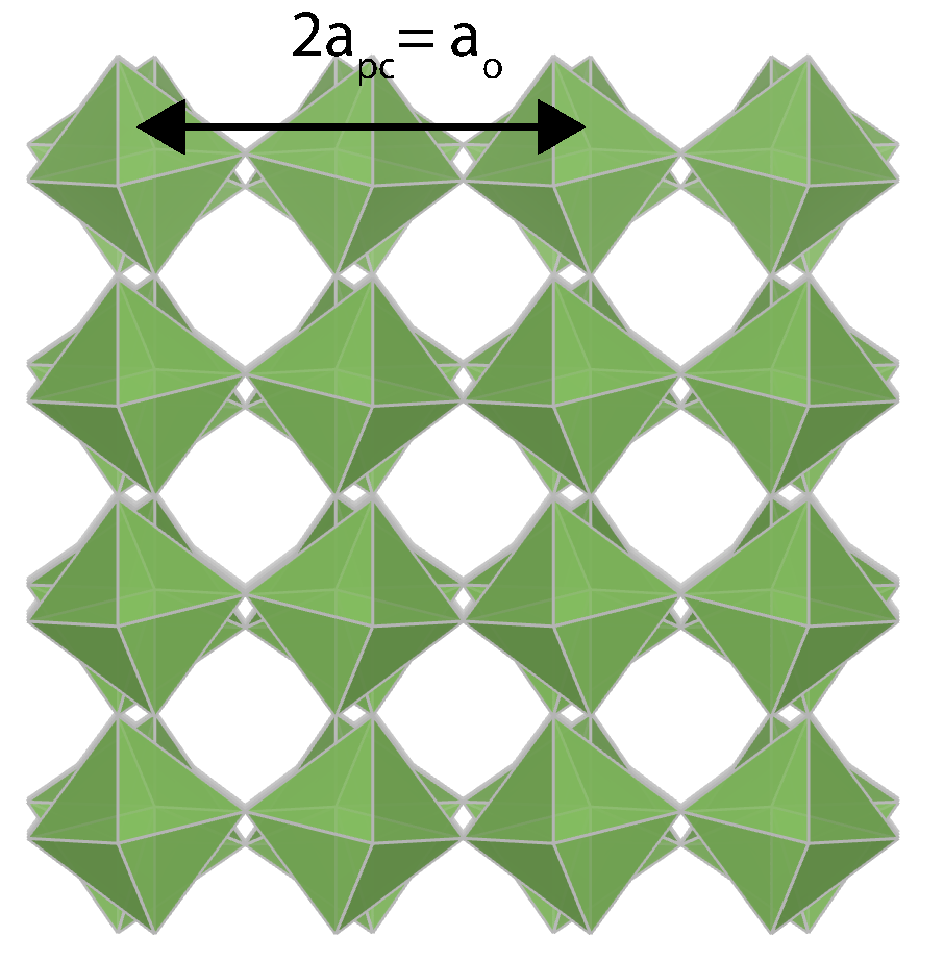
\includegraphics[width=.35\textwidth]{figures/results1/tilts_doubling.pdf}
    \caption{Doubling of the in-plane lattice parameter as a result of \ce{BO6} octahedral rotations around the out-of-plane direction}
    \label{fig:oor double symm}
\end{figure}
As a consequence of rotations about an out-of-plane axis, the material's in-plane lattice parameter has now doubled and the overall symmetry of the structure is altered.  
Octahedral rotations can be further classified as in-phase or out-of-phase.  
For out-of-phase rotations, the rotation direction about an axis changes from clockwise to counter clockwise in neighboring octahedra along the rotation axis while for in-phase rotations, the direction of rotation remains the same.  
Out-of-phase rotations therefore double the lattice parameter both parallel and perpendicular to the chosen rotation axis.  

Glazer outlined all of the possible octahedral rotation patterns for perovskites in two papers in the 1970s~\cite{Glazer1972,Glazer1975} and identified a total of 23 possible patterns.  
To classify these patterns, a three index notation was devised where each index corresponds with rotations about a particular axis with a superscript dictating in-phase versus out-of-phase rotations.  
For example, NGO takes on an $a^-b^+a^-$ octahedral rotation pattern.  
Rotations about the \hkl[1 0 0]$_{pc}$ and \hkl[0 0 1]$_{pc}$ axis are both out-of-phase, denoted by a $(-)$ superscript, and have the same rotation magnitude identified by the same letter, while rotations about the \hkl[0 1 0]$_{pc}$ axis are in-phase and have a different magnitude.  
Both LSCO and LSMO take on an $a^-a^-a^-$ tilt pattern in bulk with B-O-B bond angles of \SI{167}{\degree} and \SI{166.3}{\degree} respectively,  corresponding with average octahedral rotation angles of \SI{6}{\degree} and \SI{6.8}{\degree}~\cite{Caciuffo,Huijben2017}.  

Glazer's seminal work also outlines which rotation patterns lead to specific x-ray diffraction peaks.  
Recall that out-of-phase rotations change the lattice parameter in all three directions while in-phase rotations only change the lattice parameter in two directions.  
As a result, out-of-phase rotations create diffraction peaks with three half-order indices while peaks arising from in-phase rotations will have one integer index and three half-order indices.  
A diffraction peak \hkl(h k l) with all half order indices and $h \neq l$ is indicative of out-of-phase rotations about the $b$ axis.  
The complete set of rules is listed in Table~\ref{tab:halforder_rules}.  
\begin{table}[tb!]
\centering
\caption{Rules dictating the half order peaks observed for different types of octahedral rotations about the three principal axes, from~\cite{Glazer1975}}
\label{tab:halforder_rules}
\begin{tabular}{@{}cc@{}}
\toprule
Rotation & Peak Type \\ \midrule
$a^+$ & (h $\dfrac{\mathrm{k}}{2}$ $\dfrac{\mathrm{l}}{2}$),   $k\neq l$ \\\addlinespace
$b^+$ & ($\dfrac{\mathrm{h}}{2}$ k $\dfrac{\mathrm{l}}{2}$),   $h\neq l$ \\\addlinespace
$c^+$ & ($\dfrac{\mathrm{h}}{2}$ $\dfrac{\mathrm{k}}{2}$ l),   $h\neq k$ \\\addlinespace
$a^-$ & ($\dfrac{\mathrm{h}}{2}$ $\dfrac{\mathrm{k}}{2}$ $\dfrac{\mathrm{l}}{2}$),   $k\neq l$ \\\addlinespace
$b^-$ & ($\dfrac{\mathrm{h}}{2}$ $\dfrac{\mathrm{k}}{2}$ $\dfrac{\mathrm{l}}{2}$),   $h\neq l$ \\\addlinespace
$c^-$ & ($\dfrac{\mathrm{h}}{2}$ $\dfrac{\mathrm{k}}{2}$ $\dfrac{\mathrm{l}}{2}$),   $h\neq k$ \\\addlinespace
\bottomrule
\end{tabular}
\end{table}
With these rules in mind, a sequence of half order peaks can be selected and searched for as a way to determine a resultant octahedral tilt pattern.  
First, one of each of the in-phase rotation peaks must be identified to determine whether or not any of the octahedral rotations are in-phase.  
After the three in-phase rotation peaks have been searched for, a sequence of six out-of-phase peaks are searched for.  
Each of these peaks would correspond with two possible types of rotations and, along with the knowledge of any in-phase rotations, they can be used to rule out and deduce the resulting octahedral rotation pattern.  

A half order peak search was carried out on a \SI{15}{\nm} LSCO film on NGO substrate (C15), as well as bilayer C12M6 and single layers C12 and M6.  
A sequence of 15 peaks from sample C15, where either a substrate peak or both a film and substrate peak were observed, is shown in Figure~\ref{fig:15nm lsco half order}.  
No intensity was seen for either the film or substrate with an integer index in the $h$ or $l$ position (e.g. \hkl(0 \tfrac{3}{2} \tfrac{7}{2}) and \hkl(\tfrac{3}{2} \tfrac{7}{2} 0)), while only substrate peaks were observed when the $k$ index is at an integer value.  
This set of half order diffraction peaks confirms the expected NGO bulk octahedral pattern of $a^-b^+a^-$.  
No film peaks were observed when one of the peak indices was an integer meaning that the LSCO film is in a rotation pattern with all out-of-phase rotations, in agreement with earlier investigations of LSCO thin films~\cite{Biegalski2014}.  

A smaller subset of half order peaks was observed for single layers C12 and M6, and bilayer C12M6, shown in Figures~\ref{fig:c12 half order},~\ref{fig:m6 half order}, and~\ref{fig:c12m6 half order}.  
\begin{figure}[h!]
    \centering
    \includegraphics[width=\textwidth]{figures/results1/NA03_halforder_peaks.pdf}
    \caption{Sequence of half order peaks observed for C15}
    \label{fig:15nm lsco half order}
\end{figure}
\clearpage

\begin{figure}[h!]
    \centering
    \includegraphics[width=\textwidth]{figures/results1/C12_halforder.pdf}
    \caption{Sequence of half order peaks observed for single layer C12}
    \label{fig:c12 half order}
\end{figure}
\begin{figure}[h!]
    \centering
    \includegraphics[width=\textwidth]{figures/results1/M6_halforder.pdf}
    \caption{Sequence of half order peaks observed for single layer M6}
    \label{fig:m6 half order}
\end{figure}
\begin{figure}[h!]
    \centering
    \includegraphics[width=\textwidth]{figures/results1/C12M6_halforder.pdf}
    \caption{Sequence of half order peaks observed for bilayer C12M6}
    \label{fig:c12m6 half order}
\end{figure}
\clearpage

For both single layer C12 and bilayer C12M6, LSCO layer film peaks were observed only when all three peak indices are fractional confirming that the LSCO layer has all out-of-phase rotations.  
The observed rotation pattern for the LSCO film differs the substrate rotation pattern $a^-b^+a^-$ as well as the observed rotation pattern for $\ce{La_{0.5}Sr_{0.5}CoO3}$ thin films, $a^0b^-c^-$~\cite{Biegalski2014}.  
Some of the peaks, such as the $(\tfrac{3}{2} -\tfrac{1}{2} \tfrac{3}{2})$ were recorded in a low-resolution direction leading to the observed broadness of the substrate peak.  
No peaks from LSMO were observed for single layer M6 or bilayer C12M6, which is either due to no octahedral rotations in the LSMO layer, small octahedral rotation angles not producing a recognizable film peak, or the small LSMO film thickness producing a low signal intensity.  


\section{Quantifying Octahedral Rotations}
The octahedral rotation angles $\alpha$, $\beta$, and $\gamma$ can be experimentally determined by simulating the peak intensity of half order peaks following the procedure of May \textit{et al}~\cite{May2010}.  
A 2x2x2 perovskite super cell is constructed, only considering the 24 oxygen ion positions.  
The octahedra are then rotated by the given rotation angles, and the peak intensity is calculated using Equation~\ref{eq:peak intensity},
\begin{equation}
    I = I_0 \frac{1}{\sin (\eta)} \frac{1}{\sin(2 \Theta)} \left(\sum_{j=1}^4 D_j |F_{hkl}|^2\right)
    \label{eq:peak intensity}
\end{equation}
Where $1 / \sin(\eta)$ is a footprint correction term, $1 / \sin(2 \Theta)$ is the Lorentz polarization factor, $D_j$ is the domain fraction volume, and $F_{hkl}$ is the structure factor of the oxygen atoms calculated using Equation~\ref{eq:structure factor},
\begin{equation}
    F_{hkl} = f_{\ce{O^2-}} \sum_{n=1}^{24} \exp \left[2 \pi i \left(h u_n + k v_n + l w_n\right)\right]
    \label{eq:structure factor}
\end{equation}
where $f_{\ce{O^2-}}$ is the \ce{O^2-} form factor.  
The domain fraction term accounts for the fact that there are four possible rotation directions leading to the geometrically equivalent placement of oxygen atoms, one with all three octahedral tilt angles being positive and the other three having two positive angles and one negative angle.  
The intensity of half order peaks is determined by fitting the film and substrate peaks using a pseudo-Voigt function, and then integrating the area under the film peak.  
Intensity corrections are applied next, after which the dataset is fit for the three rotation angles.  

The outlined procedure was carried out for sample C15 which has the most comprehensive number  of half-order peak observations.  
Figure~\ref{fig:domain_peak} shows four half order peaks from the same family of planes that are used to obtain information about the domain fraction term $D_j$.  
\begin{figure}[tb!]
    \centering
    \includegraphics[width=.6\textwidth]{figures/results1/domain_peak.pdf}
    \caption{L-scans through a set of symmetrically equivalent half-order peaks}
    \label{fig:domain_peak}
\end{figure}
Peaks where the sample is rotated \SI{180}{\degree} from one another have similar shapes and intensities, while those rotated \SI{90}{\degree} from one another have different peak shapes and intensities.  
This observation is consistent with the slightly asymmetric strain state imposed by the orthorhombic NGO substrate, and suggest that there is an uneven population of the different rotational domains.  
Fitting the experimental intensity of a half order peak is simple when the film and substrate peak are separated; however, overlap between the two peaks results in inaccurate intensity values from the film peak.  
Because of this, only peaks with little to no overlap between film and substrate are used in the fitting.  
The list of peaks used for the fits is given in Table~\ref{tab:fit peak indices}.  
With this limited number of peaks, the domain fraction term $D_j$ cannot be fit, and instead fits were performed with the $D_j$ term fixed with either equal occupation for all domains, or equal population for two domains with the other having no population.  
The rotation patterns $a^0b^-c^-$, $a^-b^0c^-$, $a^-b^-c^0$, $a^-a^-c^-$, and $a^-b^-c^-$ were all simulated, and the best fit based on a $\chi^2$ goodness of fit was for a $a^-b^-c^-$ rotation pattern.  
The $\chi^2$ values for the other rotation patterns tested were approximately one order of magnitude greater than that for $a^-b^-c^-$.  
Results using either four or two equally populated domains are presented in Figures~\ref{fig:all_domain} and~\ref{fig:twodomain}.  
Because of the limited number of peaks used in the fitting, the domain fraction term is fixed during the fits.  
Using just two structural domains provides the best fit to the experimental dataset based on the lower $\chi^2$ value, with octahedral rotation angles of $\alpha = \SI{5.62}{\degree} \pm \SI{3.75}{\degree} $, $\beta = \SI{9.604}{\degree} \pm \SI{2.30}{\degree}$, and $\gamma = \SI{4.343}{\degree} \pm \SI{4.51}{\degree}$.  
The best fit values for angles $\alpha$ and $\gamma$ are slightly smaller than the bulk LSCO value of approximately $\SI{6}{\degree}$ while the angle $\beta$ is larger, although the significant amount of error associated with the calculated angles prevents a rigoruous comparions between bulk and thin film results.  
The large amount of error associated with the half order diffraction peaks arises for several different reasons.  
First, accurately extracting the intensity of a half order film peak in the immediate vicinity of the substrate peak is prone to a significant degree of error, and by investigating film peaks at higher scattering angles, where the film and substrate peak separation is higher, would be preferred.  
Furthermore, the intensity of certain half order diffraction peaks shows a strong dependence on specific octahedral rotation angles~\cite{Brahlek2017}.  
By analyzing these specific half order diffration peaks the error on half order rotation angles can be minimized.  
\begin{figure}[tb!]
    \centering
    \begin{subfigure}[t]{0.4\textwidth}
        \centering
        \includegraphics[width=\textwidth]{figures/results1/a-b-c-_all_domains.png}
        \caption{}
        \label{fig:all_domain}
    \end{subfigure}
    ~
    \begin{subfigure}[t]{0.4\textwidth}
        \centering
        \includegraphics[width=\textwidth]{figures/results1/a-b-c-_d3d4.png}
        \caption{}
        \label{fig:twodomain}
    \end{subfigure}
    \caption{Results from half order intensity fits using an $a^-b^-c^-$ rotation pattern.  $2\sigma$ error bars included on simulated dataset.  (a) Fits with four equally populated rotational domains.  (b) Fits with two equally populated rotational domains}
    \label{fig: half order fits}
\end{figure}

\begin{table}[tb!]
\centering
\caption{Peaks used for the fittings in Figure~\ref{fig: half order fits}}
\label{tab:fit peak indices}
\begin{tabular}{@{}cc@{}}
\toprule
Index & Peak \\ \midrule
0 & ($\dfrac{3}{2}$ $\dfrac{3}{2}$ $\dfrac{5}{2}$ )\\\addlinespace
1 & ($\dfrac{3}{2}$ -$\dfrac{1}{2}$ $\dfrac{5}{2}$ )\\\addlinespace
2 & ($\dfrac{3}{2}$ $\dfrac{1}{2}$ $\dfrac{5}{2}$ )\\\addlinespace
3 & ($\dfrac{3}{2}$ $\dfrac{1}{2}$ $\dfrac{7}{2}$ )\\\addlinespace
4 & ($\dfrac{5}{2}$ $\dfrac{1}{2}$ $\dfrac{7}{2}$ )\\\addlinespace
5 & ($\dfrac{5}{2}$ $\dfrac{1}{2}$ $\dfrac{3}{2}$ )\\\addlinespace
\bottomrule
\end{tabular}
\end{table}

\section{Conclusion}

Structural characterization of single layer films and LSMO / LSCO bilayers grown on NGO substrates confirms high quality film growth with experimental thicknesses in close agreement with the desired thickness.  
RSMs confirm that the films are coherently strained to the substrate with a slight distortion to one of the in-plane unit cell angles resulting in a monoclinic unit cell.  
Analysis of half-order diffraction peaks suggests that LSCO films have out-of-phase rotations about all three axes when grown both as a single layer film and as the first layer in a LSMO / LSCO bilayer.  
Best fits to the intensity of half-order peaks show that LSCO films have octahedral rotation angles of $\alpha = \SI{5.62}{\degree} \pm \SI{3.75}{\degree} $, $\beta = \SI{9.604}{\degree} \pm \SI{2.30}{\degree}$, and $\gamma = \SI{4.343}{\degree} \pm \SI{4.51}{\degree}$.  

    %!TEX root = ../main.tex
\chapter{Electronic and Magnetic Characterization of LSMO/LSCO Bilayers}
In order to monitor how interfacial charge transfer and magnetic switching behavior of LSMO / LSCO bilayers is modified by growth on \hkl(1 1 0)$_\mathrm{o}$-oriented NGO substrates, extensive electronic and magnetic characterization was performed.  
This chapter first discusses soft x-ray absorption (XA) and x-ray magnetic circular dichroism (XMCD) results from single layer LSCO, single layer  LSMO, and bilayer LSMO/LSCO on \hkl(1 1 0)$_\mathrm{o}$-oriented NGO substrates including a discussion of fits to experimental XA spectra, and is followed by a discussion of the magnetic switching behavior of these films.  

\section{Experimental Methods}
XA spectra were recorded at beamlines 6.3.1 and 4.0.2 at the Advanced Light Source.  
At beamline 6.3.1, XA spectra were recorded as the average of energy scans with right circularly polarized light in $\pm \SI{1.5}{\tesla}$ fields, while XMCD spectra were taken as the difference.  
Total electron yield (TEY) detection was utilized.  
Co L-edge spectra for samples C12, C8, C4, and C2 as well as Mn L-edge spectra for samples C12M6, C8M6, C4M6, C2M6, and M6 were measured.  
For beamline 4.0.2, XA spectra were taken by averaging energy scans with right or left circularly polarized light in a fixed field of \SI{2}{\tesla}, and both TEY and luminescence yield (LY) detection were used.   
Spectra recorded in TEY mode are representative of the top 4-10\si{\nm} of material because of the finite escape depth of electrons, while those recorded with LY detection provide information from the entire sample volume~\cite{Lee2010,Bianconi1978}.  
Co L-edge spectra for samples C12M6, C8M6, C4M6, and C2M6 were recorded at beamline 4.0.2.  
All x-ray spectra were recorded with x-rays at \SI{30}{\degree} grazing incidence with respect to the sample surface with the applied magnetic field parallel to the incident x-rays, such that the in-plane component of the applied  field was parallel to the NGO \hkl[0 0 1]$_\mathrm{o}$ direction.  

Element specific XMCD hysteresis loops were also measured at beamline 6.3.1.  
Loops at the Co L-edge were measured with $\pm \SI{1.9}{\tesla}$ fields for single layer LSCO films.  
Biased loops at the Mn L-edge were measured for bilayer LSMO/LSCO films where a \SI{1.9}{\tesla} field was applied to the sample to saturate both the soft LSMO and hard LSCO layers.  
Following the application of a saturating field, hysteresis loop were measured up to $\SI{.25}{\tesla}$ field, below the coercivity of the hard layer for bilayer C12M6.  

Major hysteresis loops were measured in a Quantum Design VersaLab physical property measurement system equipped with a vibrating sample magnetometer (VSM) attachment.  
Samples were cooled to \SI{80}{\kelvin} in zero field and the field was swept between $\pm \SI{2}{\tesla}$ while the magnetic moment was recorded.  
The VersaLab was also utilized to measure the magnetic remanence as a function of temperature.  
In these measurements, samples were cooled in a \SI{2}{\tesla} field to \SI{50}{\kelvin}.  
Next the field was set to \SI{0}{\tesla} and the sample was heated to \SI{300}{\kelvin} while the remanent magnetization was monitored.  
All VSM data was normalized to the sample area.  

\section{Soft X-Ray Spectroscopy}
Experiments performed with LSMO/LSCO bilayers on LSAT substrates indicate that a \ce{Co^2+} ion-rich sublayer forms within the LSCO layer close to the LSMO/LSCO interface as a result of charge transfer from LSMO to LSCO~\cite{Li2014}.  
The interfacial sublayer was found to be magnetically soft and strongly coupled with the LSMO layer instead of the hard LSCO layer.  
In order to determine how growth on an orthorhombic substrate with octahedral tilts (\hkl(1 1 0)$_\mathrm{o}$-oriented NGO) impacts charge transfer and formation of the interfacial sublayer, extensive XA spectroscopy  and XMCD measurements were performed at the Co and Mn L-edges.  
\begin{figure}[tb!]
    \centering
    \includegraphics[width=.6\textwidth]{figures/results2/Mn_80k_xas_xmcd_ey.pdf}
    \caption[Mn L-Edge XA and XMCD spectra from LSMO/LSCO bilayers taken at 80K]{Mn L-edge XA and XMCD spectra from LSMO/LSCO bilayers and single layer M6 taken at 80K, acquired in TEY mode. XA spectra shifted vertically for clarity.}
    \label{fig:mn_xas}
\end{figure}
Figure~\ref{fig:mn_xas} plots the experimentally measured Mn L-edge XA and XMCD spectra for all LSMO/LSCO bilayers and includes single layer M6 for comparison.  
XA spectra for all bilayers show close resemblance to sample M6 where the Mn valence state is a mixture of \ce{Mn^4+}/\ce{Mn^3+} ions.  
Charge transfer between individual layers should lead to a change in Mn valence which is accompanied by L$_3$ and L$_2$ peak shifts and changes to spectral shapes; however, no significant differences were observed amongst the Mn spectra.  
The shape of the bilayer LSMO/LSCO XMCD spectra in Figure~\ref{fig:mn_xas} resemble that of single layer M6 indicating that magnetism in the LSMO layer arises from a double exchange interaction between \ce{Mn^3+} and \ce{Mn^4+} ions.  
XMCD spectra for the bilayer samples all have the same magnitude as single layer spectra indicating that the LSMO layer magnetization is constant with changing LSCO layer thickness.  

Experimental Co L-edge XA and XMCD spectra in TEY mode for the LSMO/LSCO bilayers are plotted in Figure~\ref{fig:co_xas_xmcd_ey}.  
Reference spectra from \ce{Co^3+} ions (\ce{LaCoO3}), mixed \ce{Co^3+}/\ce{Co^4+} ions (LSCO), and \ce{Co^2+} ions (\ce{La2CoMnO6}) are also included.  
\begin{figure}[tb!]
    \centering
    \includegraphics[width=.6\textwidth]{figures/results2/Co_bilayer_80k_xmcd_EY.pdf}
    \caption[Co L-Edge XMCD spectra from LSMO/LSCO bilayer taken at \SI{80}{\kelvin} with TEY detection]{Co L-Edge XA and XMCD spectra from LSMO/LSCO bilayers taken at \SI{80}{\kelvin} in TEY mode, with representative reference spectra.  Features A and B denote prominent features associated with \ce{Co^2+} ions and  feature C corresponds with the XA peak from mixed \ce{Co^3+}/\ce{Co^4+}.  Best fits to experimental spectra using Equation~\ref{eq:3_ref} are overlaid in black. XMCD spectra normalized to the absolute value of their minimum}
    \label{fig:co_xas_xmcd_ey}
\end{figure}
Several prominent spectral features are labeled, where features A and B are representative of \ce{Co^2+} ions and feature C corresponding to the mixed \ce{Co^3+}/\ce{Co^4+} L$_3$ peak position.  
Bilayers C12M6 and C8M6 closely resemble the LSCO reference with their L$_3$ peak lining up with feature C, indicating that Co ions are in a mixed \ce{Co^3+}/\ce{Co^4+} valence state in these two films.  
XMCD spectra for C12M6 and C8M6 were also found to be similar in shape to the reference LSCO XMCD spectra, confirming that LSCO layer magnetism arises from double exchange between the mixed valence \ce{Co} ions.  
The Co XA spectra for bilayers C4M6 and C2M6 differ from the two thicker bilayers showing features characteristic of \ce{Co^2+} ions - the L$_2$ peak becomes highly asymmetric while the L$_3$ peak shifts to lower energies and shows a complex multiplet structure.  
The observed spectral changes for the two thinnest bilayers are representative of charge transfer from the LSMO layer to the LSCO layer.  
XMCD spectra for bilayers C4M6 and C2M6 show a small positive peak and large negative peak lining up with the reference \ce{La2CoMnO6} XMCD spectra indicating that the \ce{Co^2+} ions are magnetically active.  

The Co XA and XMCD spectra in Figure~\ref{fig:co_xas_xmcd_ey} were taken in TEY mode and therefore give information primarily from the LSCO layer close to the LSMO interface where charge transfer occurs.  
Spectra were also recorded in LY mode giving information from throughout the volume of the LSCO layer.  
LY spectra are shown in Figure~\ref{fig:co_xas_ly}.  
The LY efficiency of the NGO substrates is very small resulting in a low signal-to-noise ratio especially for the thinnest LSCO samples and XMCD measurements.  
For this reason, XMCD spectra in LY mode are not shown.  
\begin{figure}[tb!]
    \centering
    \includegraphics[width=.6\textwidth]{figures/results2/Co_bilayer_80k_xmcd_LY.pdf}
    \caption[Co L-Edge XA spectra from LSMO/LSCO bilayers taken at \SI{80}{\kelvin} with LY detection]{Co L-Edge XA spectra from LSMO/LSCO bilayers taken at \SI{80}{\kelvin} with LY detection, with representative reference spectra (* denotes TEY detection).  Best fits overlaid in black.  Features A and B denote prominent features associated with \ce{Co^2+} ions and  feature C corresponds with the XA peak from mixed \ce{Co^3+}/\ce{Co^4+}.}
    \label{fig:co_xas_ly}
\end{figure}
LY Co L-edge XA spectra for bilayers C12M6 and C8M6 closely resemble the TEY spectra with their L$_3$ peak lining up with that of the LSCO reference.  
As the Co layer thickness decreases, features A and B begin to grow, although to a lesser extent than in the TEY spectra.  
The complex multiplet structure observed in TEY spectra is also not present and instead bilayers C4M6 and C2M6 are closer in shape to the \ce{Co^3+} \ce{LaCoO3} reference.  
MEPS increases the amount of \ce{Co^3+} ions compared with \ce{Co^4+} ions in close proximity to the substrate interface, a volume of material that is only probed in LY mode for the LSMO/LSCO bilayers.  
XA spectra for single layer LSCO films in Figure~\ref{fig:co_80k_xa_xmcd_single}, taken in TEY mode, also resemble the \ce{LaCoO3} for thickness \SI{4}{\nm} and below, in agreement with measurements performed for similar films on LSAT substrates~\cite{Li2017b}.  
The two thicker LSCO films closely resemble the LSCO reference spectra.  
\begin{figure}[tb!]
    \centering
    \includegraphics[width=.6\textwidth]{figures/results2/Co_single_80k_xmcd_ey.pdf}
    \caption[Co L-edge XA and XMCD spectra from single layer Co samples taken at 80K]{Co L-edge XA and XMCD spectra taken at 80K from single layer Co samples in TEY mode, compared with reference spectra representative of mixed \ce{Co^3+}/\ce{Co^4+} (LSCO) and \ce{Co^3+} (\ce{LaCoO3}) valence states.  Black lines show the best fit to experimental data, taken as the linear combination of reference spectra in Equation~\ref{eq:3_ref}.  Samples C4 and C2 showed extensive charging effects and their XMCD spectra are not shown.}
    \label{fig:co_80k_xa_xmcd_single}
\end{figure}
No \ce{Co^2+} ion formation is observed for the single layer samples confirming that its formation depends on the presence of an LSMO overlayer.  
XMCD spectra for single layers C12 and C8 closely resemble the LSCO reference, while single layers C4 and C2 showed significant charging effects and their XMCD spectra are therefore not shown.  

\section{X-Ray Absorption Spectra Fitting}
To extract quantitative information about ionic valence changes and better compare XA results between different samples and detection modes, experimental spectra were fit using a linear combination of reference spectra.  
To perform the fits, experimental spectra must first have their background removed.  
The background is given by a step function convoluted with a Gaussian, which is estimated by an error function~\cite{vanderLaan2014}.  
For a pure metal sample, background subtraction is relatively straightforward: the background shows two jumps as it passes through the L$_3$ and L$_2$ peaks, with the L$_3$ background height being double that of the L$_2$ height.  
The total height of the jump can be taken as the signal intensity after any extended absorption oscillations have subsided, which occurs approximately 20-30\si{\eV} beyond the L-edge~\cite{Chen1995a}.  
The presence of \ce{La} ions in LSCO complicates the analysis because the \ce{La} M-edge is only \SI{40}{\eV} away from the \ce{Co} L-edge and the absorption effects at either edge cannot be isolated.  
For the purposes of this work, the first jump extends from the pre-edge to the XA intensity between the L$_3$ and L$_2$ peaks, and the second background jump goes up to the height of the post edge, as depicted in Figure~\ref{fig:xa_backsub_example} for the Co XA spectrum from bilayer C12M6.  
\begin{figure}[tb!]
    \centering
    \includegraphics[width=.6\textwidth]{figures/results2/backsub_example.pdf}
    \caption[Example of XAS Background Subtraction]{Background subtraction for bilayer C12M6.  Two stitched error functions are used to estimate the background.}
    \label{fig:xa_backsub_example}
\end{figure}
It is also crucial to ensure that there are no energy shifts present between experimental and reference spectra which is done by lining up prominent spectral features amongst experimental and reference spectra.  

Two different linear combinations of reference spectra were used to fit the XA spectra:
\begin{align}
    I &= A \times I_\mathrm{LSCO} + (1-A) \times I_{\ce{La2CoMnO6}} \label{eq:2_ref}\\
    I &= A \times I_\mathrm{LSCO} + B \times I_{\ce{La2CoMnO6}} + C \times I_{\ce{LaCoO3}} \label{eq:3_ref}
\end{align}
where Equation~\ref{eq:3_ref} adds sensitivity to pure \ce{Co^3+} valence compared with Equation~\ref{eq:2_ref}.  
Fit results using Equation~\ref{eq:3_ref} are overlaid as black curves in Figures~\ref{fig:co_xas_xmcd_ey},~\ref{fig:co_xas_ly}, and~\ref{fig:co_80k_xa_xmcd_single}.  
Using all three reference spectra results in better fits for all samples measured based on a $\chi^2$ test as shown in Table~\ref{tab:goodness_of_fit}.  
\begin{table}[tb]
\centering
\caption{Goodness of fit values for XA spectra fitting of single layer LSCO and bilayer LSMO/LSCO samples, simulated with either two reference spectra (equation~\ref{eq:2_ref}) or three reference spectra (equation~\ref{eq:3_ref}).}
\label{tab:goodness_of_fit}
\begin{tabular}{@{}llllllllll@{}}
\toprule
&& \multicolumn{2}{c}{Single Layer} && \multicolumn{2}{c}{Bilayer TEY} && \multicolumn{2}{c}{Bilayer LY}\\
\cmidrule{3-4} \cmidrule{6-7} \cmidrule{9-10}
LSCO Thickness && $\chi^2$ (\ref{eq:2_ref}) & $\chi^2$ (\ref{eq:3_ref}) && $\chi^2$ (\ref{eq:2_ref}) & $\chi^2$ (\ref{eq:3_ref}) && $\chi^2$ (\ref{eq:2_ref}) & $\chi^2$ (\ref{eq:3_ref}) \\ 
\hline
\SI{12}{\nm} && 0.204 & 0.174 && 0.238 &  0.221 && 0.483 & 0.470 \\
\SI{8}{\nm} && 0.278 & 0.198 && 0.150 & 0.148 && 0.314 & 0.292 \\
\SI{4}{\nm} && 0.649 & 0.192 && 0.233 & 0.148 && 0.274 & 0.208 \\
\SI{2}{\nm} && 2.72 & 0.472 && 0.464 & 0.193 && 1.99 & 0.940 \\
\bottomrule
\end{tabular}
\end{table}
Fits for samples with LSCO thicknesses of \SI{2}{\nm} and \SI{4}{\nm} show the largest change when incorporating all three reference spectra, in agreement with the qualitative observation that the \ce{Co^3+}/\ce{Co^4+} ratio increases as LSCO thickness decreases below \SI{8}{\nm}~\cite{Li2017b}.  

Figure~\ref{fig:fit_weights} presents the weight of the different reference spectra using Equation~\ref{eq:3_ref} for the bilayer spectra in TEY and LY mode, as well as singe layer spectra in TEY mode.  
\begin{figure}[tb!]
\centering
    \begin{subfigure}[b]{0.45\textwidth}
         \centering
         \includegraphics[width=\textwidth]{figures/results2/lsco_lcmo_lco_weights.pdf}
         \caption{Bilayer LSMO/LSCO, TEY.}
         \label{fig:weights_bilayerTEY}
    \end{subfigure}
    \hfill
    \begin{subfigure}[b]{0.45\textwidth}
         \centering
         \includegraphics[width=\textwidth]{figures/results2/LY_lsco_lcmo_lco_weights.pdf}
         \caption{Bilayer LSMO/LSCO, LY.}
         \label{fig:weights_bilayerLY}
    \end{subfigure}
    \\
    \begin{subfigure}[b]{0.45\textwidth}
         \centering
         \includegraphics[width=\textwidth]{figures/results2/lsco_lcmo_lco_singlelayer_weights.pdf}
         \caption{Single layer LSCO, TEY.}
         \label{fig:weights_co_single}
    \end{subfigure}
\caption[Spectral weights for XAS fits]{Spectral weights for XAS fits using Equation~\ref{eq:3_ref}.}
\label{fig:fit_weights}
\end{figure}
Results from the fits for single layer LSCO films show a transfer of weight from the \ce{Co^3+} ion reference to the LSCO reference as the LSCO layer thickness increases, with little \ce{Co^2+} ion signal.  
The large amount of \ce{Co^3+} ion weight for single layer C2 confirms substrate-induced MEPS, while the reduction in \ce{Co^3+} ion intensity with increasing thickness is an effect of the finite sample volume of TEY mode.  
As the LSCO thickness increases a \ce{Co^3+}/\ce{Co^4+} layer forms reducing the volume of MEPS layer probed by TEY detection.  

The results from fitting the TEY spectra for bilayers in Figure~\ref{fig:weights_bilayerTEY} agree with qualitative observations suggesting formation of \ce{Co^2+} ions when the LSCO thickness decreases below \SI{8}{\nm}.  
Weights of the \ce{Co^2+} reference decrease from $0.78$ for C2M6 to $0.55$ for C4M6, and reaches zero for C8M6.  
The LSCO reference weight follows an opposite trend, increasing from 0 for C2M6 to \SI{.97}{} for C8M6.  
Fits of LY spectra in Figure~\ref{fig:weights_bilayerLY} are similar to results from the TEY spectra, being predominantly LSCO-like with no \ce{Co^2+} formation and small amounts of \ce{Co^3+}.  
Differences in reference spectra weights between TEY and LY mode are apparent for the two thinner bilayers.  
The \ce{Co^3+} weight for bilayer C2M6 is \SI{50}{\percent} larger for the fits using LY spectra while the \ce{Co^2+} weight is \SI{60}{\percent} lower.  
Bilayer C4M6 also shows a large reduction in \ce{Co^2+} weight, but this difference is balanced by an increase in the LSCO weighting with no change in \ce{Co^3+} for the LY spectra fits indicating formation of a \ce{Co^3}/\ce{Co^4+} layer.  
These differences between LY and TEY spectra arise because of the different sample volumes probed, with LY spectra being representative of a the entire LSCO sublayer volume gaining sensitivity to the LSCO/substrate interface.  

Summarizing the fitting results, single layer LSCO splits into multiple layers with a non-magnetic MEPS layer at the LSCO-substrate interface.  
For single layer C2 there is only a MEPS layer present, while for LSCO layer thicknesses of \SI{4}{\nm} and  above an additional mixed valence \ce{Co^3+}/\ce{Co^4+} LSCO layer is also present with magnetism mediated by an double exchange.  
The LSCO layer in LSMO / LSCO bilayers displays different behavior as a function of thickness.  
Bilayer C2M6 has two LSCO layers with MEPS at the LSCO-substrate interface and a \ce{Co^2+} ion-rich magnetically active interfacial layer.  
For bilayer C4M6 an additional LSCO layer forms between the MEPS and \ce{Co^2+} ion-rich layer.  
Interestingly, the \ce{Co^2+} interfacial layer is not present for bilayers C8M6 and C12M6, even based on TEY detection data which is most sensitive to the LSMO / LSCO interfacial region.  
These results for bilayers are in contrast with similar experiments performed on LSAT substrates that show a more gradual reduction in the \ce{Co^2+} ion-rich layer as a function of increasing LSCO layer thickness, persisting for LSCO layer thicknesses of \SI{8}{\nm}~\cite{Li2016,Kane2019}.  

\section{Magnetometry}
Major hysteresis loops were measured for all bilayers as well as single layers C12, C8, and M6 at \SI{80}{\kelvin} to a  $\pm \SI{2}{\tesla}$ measuring field along the NGO \hkl[0 0 1]$_\mathrm{o}$ direction to ensure saturation of both magnetic layers.  
Single layers C4 and C2 were found to be non-magnetic and no hysteresis loop were observed.  
Hysteresis loops were normalized to the sample area unless otherwise noted.  
The remanent magnetization, $M_r$, was also tracked as a function of temperature.  
Typical magnetization versus temperature measurements that apply a small measuring field are difficult to perform for films on NGO substrates because of their large paramagnetic moment and therefore the remanent magnetization was tracked as a function of temperature.  
The $M_r(T)$ data was collected by cooling the sample in a field \SI{2}{\tesla} parallel to the NGO \hkl[0 0 1]$_{\mathrm{o}}$ direction and measuring the magnetic moment in zero applied field while the sample is heated.  

The T-dependence of $M_r$ is shown in Figure~\ref{fig:bilayer_tmr} for all four bilayers as well as single layers M6, C12, and C8.  
\begin{figure}[tb!]
    \centering
    \includegraphics[width=.7\textwidth]{figures/results2/bilayer_tmr.pdf}
    \caption[Remanent magnetization versus temperature]{Remanent magnetization versus temperature for LSMO/LSCO bilayer series and single layers M6, C12, and C8.  Cooling field and magnetization measured along the NGO \hkl[0 0 1]$_\mathrm{o}$ direction.}
    \label{fig:bilayer_tmr}
\end{figure}
Similar profiles were observed for all measurements except that of bilayer C2M6 which shows little magnetization for all measured temperatures.  
A sharp drop to negative remanence was seen as the temperature was raised to a critical value.  
This drop to negative magnetization may be attributed to small amounts of trapped flux in the magnet yoke.  
When temperature is increased to approach $T_c$, the coercive field typically decreases~\cite{Lee2017} and eventually any small amount of trapped flux is able to reverse the sample magnetization leading to a negative $M_r$.  

A critical temperature can be defined for the $M_r$ data as the point where $dM_r/dT$ is at a maximum.  
Values are reported in Table~\ref{tab:bialyer_tc_tmr} for all samples.  
\begin{table}[tb!]
    \centering
    \caption{Critical Temperature extracted from $M_r$ temperature dependence.}
    \begin{tabular}{ll}
    \toprule
    Sample & T$_\mathrm{c}$ (\si{\kelvin})    \\ \hline
    C12M6  & 194.7 \\ 
    C12 & 190.7 \\
    C8M6   & 180.8 \\ 
    C8 & 174.9 \\
    C4M6   & 239.5 \\ 
    C2M6 & 123.6 \\
    M6     & 270.0 \\ 
    \bottomrule
    \end{tabular}
    \label{tab:bialyer_tc_tmr}
\end{table}
For bilayer C12M6, the critical point occurs \SI{4}{\kelvin} above single layer C12 and for bilayer C8M6 it occurs \SI{5.9}{\kelvin} above that of single layer C8.  
Interestingly the remanent magnetization for bilayers drops to zero at the critical temperature.  
A small amount of remanent magnetization associated with the LSMO layer may be expected to persist above the critical temperature for the bilayer samples as hysteresis loops recorded at \SI{80}{\kelvin} and \SI{250}{\kelvin} for bilayer C12M6, shown in Figure~\ref{fig:c12m6_Temploops}, indicate that the two thicker bilayer samples are still magnetic above their single reported critical temperatures with the second hard magnetic transition at \SI{0.6}{\tesla} only occurring below \SI{80}{\kelvin}.  
These hysteresis loop results suggest that the critical temperatures recorded for bilayers C12M6 and C8M6 are the temperatures at which the LSCO layer becomes nonmagnetic.  

Bilayer C4M6 differs from the two thicker bilayer samples with a critical temperature within \SI{40}{\kelvin} of the critical temperature for M6.  
XA and XMCD results indicate that bilayer C4M6 forms a magnetically active \ce{Co^2+} ion-rich interfacial layer which may account for this difference.  
Bilayer C2M6 has a very weak remanent magnetization with a low critical temperature of \SI{123.6}{\kelvin}.  
\begin{figure}[tb!]
\centering
\begin{subfigure}[b]{0.45\textwidth}
         \centering
         \includegraphics[width=\textwidth]{figures/results2/80k_250k_na08_loops.pdf}
         \caption{C12M6}
         \label{fig:c12m6_Temploops}
     \end{subfigure}
     ~
     \begin{subfigure}[b]{0.45\textwidth}
         \centering
         \includegraphics[width=\textwidth]{figures/results2/c4m6_temp_loops.pdf}
         \caption{C4M6}
         \label{fig:c4m6_temploops}
     \end{subfigure}
\caption{(a) Hysteresis loops for bilayer C12M6 at \SI{80}{\kelvin} and \SI{250}{\kelvin}.  Magnetic field applied along the NGO \hkl[1 -1 0]$_{o}$ direction (b) Hysteresis loops for bilayer C4M6 at \SI{80}{\kelvin}, \SI{225}{\kelvin}, and \SI{300}{\kelvin}.  Magnetic field applied along the NGO \hkl[0 0 1]$_{o}$ direction}
\label{fig:bilayer_temp_loops}
\end{figure}
Hysteresis loops for bilayer C4M6 in Figure~\ref{fig:c4m6_temploops} show that it is non-magnetic above the critical temperature of \SI{239.5}{\kelvin} confirming that for this bilayer the critical temperature represents the magnetic transition for both layers.  
Coincident loss of magnetization in both the LSMO and LSCO layers in bilayer C4M6 suggests that the two layers are magnetically coupled, as does the observation that the hysteresis loop for C4M6 at \SI{80}{\kelvin} shows just one magnetic transition.  
An interfacial layer with magnetically active \ce{Co^2+} ions, shown to be present in bilayer C4M6 by XA and XMCD spectroscopy, tends to couple strongly to the LSMO layer~\cite{Li2014}.  

Major hysteresis loops were recorded for all LSMO/LSCO bilayers as well as single layers C12 and C8 in order to track how magnetic switching varies as a function of LSCO thickness.  
In a VSM measurement, the recorded dataset is a combination of all of the magnetic signals present in the chamber including those from the thin films of interest and the substrate.  
NGO substrates have a strong paramagnetic signal because of the \ce{Nd} ions and it is often reported that VSM magnetometry is not possible for thin films grown on this substrate~\cite{Bolstad2018}, but the results in this thesis suggest that this is not necessarily true.  

In Figure~\ref{fig:loop_backsub} the background subtraction process is illustrated using single layer C12 as a representative example.  
\begin{figure}[tb]
\centering
\begin{subfigure}[b]{0.45\textwidth}
         \centering
         \includegraphics[width=\textwidth]{figures/results2/loop_backsub_example.pdf}
         \caption{}
         \label{fig:loop_backsub}
     \end{subfigure}
     ~
     \begin{subfigure}[b]{0.45\textwidth}
         \centering
         \includegraphics[width=\textwidth]{figures/results2/c12_xmcd_loop_001.pdf}
         \caption{}
         \label{fig:c12_xmcd_loop}
     \end{subfigure}
\caption{(a) Background subtraction procedure for single layer C12.  
        (b) C12 Co XMCD hysteresis loop.  Magnetic field applied along NGO \hkl[0 0 1]$_{o}$ direction}
\label{fig:backsub_xmcd_loop}
\end{figure}
First the raw data (red line) is fit to a straight line and subtracted from the dataset, resulting in the blue curve which shows an unexpected soft magnetic transition at low fields.  
A small residual ferromagnetic signal from either the substrate or VSM chamber is responsible for the observed soft switching event, gathered by running an identical scan on a \ce{Pd} reference standard and subtracting away the \ce{Pd} paramagnetic moment.  
Ideally this scan would be performed on an identical piece of NGO.  
When the residual ferromagnetic signal is removed, the green curve in Figure~\ref{fig:loop_backsub} is recovered showing a single hard switching event for single layer C12.  
The Co elemental specific hysteresis loop in Figure~\ref{fig:c12_xmcd_loop} justifies subtraction of a residual loop because it only shows a single hard magnetic transition with a coercivity of \SI{0.70}{\tesla}.  
Data divergence at high magnetic fields for the XMCD hysteresis loop is attributed to interactions between the changing magnetic field and the captured TEY and I0 normalization signals.  
After background subtraction the coercive field obtained from VSM measurements for single layer C12 is \SI{0.75}{\tesla}, in close agreement with the value extracted from XMCD loops.  

Hysteresis loops for singe layers C12 and C8 are plotted in Figure~\ref{fig:loops_single_layer}.  
\begin{figure}[tb!]
    \centering
    \includegraphics[width=\textwidth]{figures/results2/single_loops_final.pdf}
    \caption{Hysteresis loops for single layer LSCO at \SI{80}{\kelvin} measured in a VSM (left panel) and XMCD hysteresis loops at the Co L-edge (right panel).  Magnetic field applied along the NGO \hkl[0 0 1]$_{o}$ direction}
    \label{fig:loops_single_layer}
\end{figure}
The background subtraction procedure successfully removed the soft magnetic transition for single layer C12 but did not work completely for single layer C8, and therefore assuming a constant background amongst different samples is not completely accurate.  
Instead, each substrate piece should be measured for background subtraction prior to film growth in order to account for magnetic differences amongst substrate pieces although doing so risks surface contamination which negatively impacts film growth.  
In this way, an accurate background value can be determined for each sample.   
Single layer C8 shows a soft transition with a coercivity of \SI{0.02}{\tesla} and a hard transition with a coercivity of \SI{.32}{\tesla}.  
This hard magnetic transition is also present in the XMCD loop at the same coercive field.  

Remanence values for single layer C12 agree with the values from the temperature dependence in Figure~\ref{fig:bilayer_tmr}, whereas the remanence value extracted from the loops for C8 is double that of the value from the temperature dependent measurements.  
The observed discrepancy in $M_r$ between the hysteresis loop and the $M_r$ versus T data is another indicator that the background removal attempts were not successful for single layer C8.  

Versalab loops for all four bilayers are presented in Figure~\ref{fig:bilayer_vsm_loops}.  
\begin{figure}[tb!]
    \centering
    \includegraphics[width=\textwidth]{figures/results2/bilayer_loops_final.pdf}
    \caption[Versalab Hysteresis loops for LSMO/LSCO bilayers]{Hysteresis loops for LSMO/LSCO bilayers measured at \SI{80}{\kelvin}.  Magnetic field applied along the NGO \hkl[0 0 1]$_{o}$ direction}
    \label{fig:bilayer_vsm_loops}
\end{figure}
The hysteresis loop for bilayer C12M6 shows two switching events, a soft switching event at \SI{.077}{\tesla} corresponding with the LSMO layer and a hard switching event at \SI{0.6}{\tesla} which is \SI{0.15}{\tesla} lower than the coercivity for single layer C12.  
Bilayer C8M6 also shows two switching events with similar coercive fields while bilayers C4M6 and C2M6 show just one magnetic switching event.  
Bilayer C4M6 has a square hysteresis loop and a large $M_r$ while bilayer C2M6 has negligible remanence consistent with a magnetic hard direction.  
Magnetic remanence trends from hysteresis loops of LSMO/LSCO bilayers are consistent with those from $M_r$ as a function of temperature: as the LSCO sublayer thickness decreases $M_r$ also decreases being close to zero for \SI{2}{\nm} LSCO layer thickness.  
Saturation magnetization for bilayer C8M6 is larger than that for C12M6 while it is nearly the same for bilayers C4M6 and C2M6 even though areal normalized $M_s$ values should scale with total film thickness.  
Mn L-edge XMCD measurements show identical XMCD signal from these two bilayers indicating that the discrepancy in saturation magnetization is due to contributions from the LSCO layer.  
The Co L-edge XMCD maximum in TEY mode for bilayer C4M6 is only \SI{10}{\percent} smaller than that of bilayer C2M6, therefore the interfacial layer cannot be responsible for the observed difference.  

Hysteresis loops measured on LSAT substrates for bilayers C12M6 and C8M6 show two distinct magnetic transitions with the soft magnetic transition occurring at \SI{.0006}{\tesla} for C8M6 and \SI{.0009}{\tesla} for C12M6, significantly lower than that for the same bilayers on NGO substrates.  
The hard switching event for bilayer C12M6 on LSAT and NGO substrates occurs at roughly the same switching field of \SI{.6}{\tesla}.  
There are also distinct differences between the two substrates for the thinner bilayers.  
On LSAT substrates the loop shape for bilayers C4M6 and C2M6 are the same showing a single soft switching event representative of strong magnetic coupling between the LSCO and LSMO layers~\cite{Wynn2015}.  
Hysteresis loops for these two bilayers on NGO substrates also show a single switching event but bilayer C2M6 has little remanence along the \hkl[0 0 1]$_\mathrm{o}$ direction.  
The ratio between the remanent magnetization and the saturation magnetization, referred to as the loop squareness, is given for LSMO/LSCO bilayers on NGO and LSAT substrates in Figure~\ref{tab:bialyer_mr/ms}.    
\begin{table}[tb!]
    \centering
    \caption{$M_r / M_s$ ratio for the LSMO/LSCO bilayer hysteresis loops in Figure~\ref{fig:bilayer_vsm_loops}}
    \begin{tabular}{lll}
    \toprule
    Sample & $M_r / M_s$ (NGO) &  $M_r / M_s$ (LSAT)~\cite{Wynn2015}  \\ \hline
    C12M6  & 0.652 & 0.59\\ 
    C8M6   & 0.469 & 0.84\\ 
    C4M6   & 0.942 & 0.45\\ 
    C2M6   & 0.256 & 0.60\\ 
    \bottomrule
    \end{tabular}
    \label{tab:bialyer_mr/ms}
\end{table}
The loop squareness is a useful comparison for comparing how hard or soft a magnetic transition is, with a small value indicating a magnetically hard direction.  
No obvious trend exists for the loop for bilayers on NGO and LSAT substrates suggesting that multiple different competing factors control magnetic switching in LSMO/LSCO bilayers.  

\section{Magnetocrystalline Anisotropy}
Hysteresis loops were measured for bilayer C12M6 with the field applied parallel to the \hkl[1 0 0]$_{pc}$, [0 1 0]$_{pc}$, and [1 1 0]$_{pc}$ directions, while XMCD hysteresis loops, were recorded along the \hkl[1 0 0]$_{pc}$ and \hkl[1 1 0]$_{pc}$ directions for single layers C12, C8, and M6 to study magnetocrystalline anisotropy in films on NGO substrates.  
The loops for bilayer C12M6, shown in Figure~\ref{fig:c12m6_anisotropy_loops}, have different shapes when measured along the \hkl[1 0 0 ]$_{pc}$ direction compared with the  \hkl[0 1 0]$_{pc}$ and \hkl[1 1 0]$_{pc}$ directions.  
\begin{figure}[tb]
    \centering
    \includegraphics[width=.5\textwidth]{figures/results2/c12m6_anisotropy.pdf}
    \caption{Hysteresis loops for bilayer C12M6 measured at \SI{80}{\kelvin} with the magnetic field applied parallel to the labeled direction}
    \label{fig:c12m6_anisotropy_loops}
\end{figure}
When the field is applied parallel to the \hkl[1 0 0]$_{pc}$ direction, the hard transition at \SI{.58}{\tesla} corresponding with the LSCO layer is significantly sharper compared with the very gradual transition measured along the other two pseudocubic directions.  
These results for bilayer C12M6 suggest a \hkl[1 0 0]$_{pc}$ easy direction.  

Co L-edge XMCD hysteresis loops for single layers C12 and C8 are shown in Figure~\ref{fig:xmcd_singlelayer_loops}.  
All of the loops show nonlinear behavior at high fields which is attributed to the changing magnetic field altering the raw TEY detection signal.  
Furthermore, the I0 incident beam intensity normalization signal shows unexpected magnetic field dependence which further alters the loop behavior at high fields.  
\begin{figure}[tb]
\centering
    \begin{subfigure}[tb]{.49\textwidth}
        \centering
        \includegraphics[width=\textwidth]{figures/results2/c12_xmcd_loop_anisotropy.pdf}
        \caption{}
        \label{fig:c12_xmcd}
    \end{subfigure}
    ~
    \begin{subfigure}[tb]{.49\textwidth}
        \centering
        \includegraphics[width=\textwidth]{figures/results2/c8_xmcd_loop_anisotropy.pdf}
        \caption{}
        \label{fig:c8_xmcd}
    \end{subfigure}
\caption{Co XMCD hysteresis loops for (a) C12 and (b) C8.  Legend denotes direction of applied magnetic field.}
\label{fig:xmcd_singlelayer_loops}
\end{figure}
For both C12 and C8 a single hard switching event was observed for both measured orientations.  
In C12 and C8 there is a \SI{20}{\percent} reduction in the coercive field between the \hkl[1 0 0]$_\mathrm{pc}$ and \hkl[1 1 0]$_\mathrm{pc}$  directions suggesting a \hkl[1 1 0]$_\mathrm{pc}$ easy direction.  
The shape of XMCD spectra does not change for different orientations, while a \SI{30}{\percent} reduction in the XMCD maximum is observed along the \hkl[1 1 0] direction for both single layers C12 and C8.  
Furthermore the coercive field decreases as the LSCO thickness decreases.  
These observations are consistent with the thickness and orientation trends in coercivity for single layer LSCO on LSAT substrates~\cite{Wynn2015}.   

The Mn L-edge XMCD loops for single layer M6 are shown in Figure~\ref{fig:m6_xmcD_loop}.  
Mn XA and XMCD spectra are identical in shape and magnitude along the two measured directions for single layer M6.  
A single magnetic transition is observed along both directions, and the loop shape is nearly identical.  
\begin{figure}[tb]
    \centering
    \includegraphics[width=.5\textwidth]{figures/results2/m6_xmcd_loop_anisotropy.pdf}
    \caption{Mn XMCD Hysteresis loop for single layer M6.  Legend denotes direction of applied magnetic field}
    \label{fig:m6_xmcD_loop}
\end{figure}
Furthermore, no change in coercivity occurs indicating a lack of magnetocrystalline anisotropy.  
This observation is in direct contrast to films on NGO and LSAT substrates.   
\SI{18}{\nm} LSMO films on NGO possess a \hkl[1 0 0]$_\mathrm{pc}$ easy direction and a \hkl[0 1 0] hard direction~\cite{Matthews2007}.  
LSMO on LSAT substrates show uniaxial magnetic anisotropy with a \hkl[1 1 0] easy direction and a \hkl[1 0 0] hard direction, although the anisotropy is not strong~\cite{Monsen2014}.  

Summarizing the magnetocrystalline anisotropy results, bilayer C12M6 has a \hkl[1 0 0]$_{pc}$ easy direction.  
In contrast, single layers C12 and C8 have a \hkl[1 1 0]$_{pc}$ easy direction while single layer M6 does not have anisotropic magnetic behavior.  
These results show that both film thickness and the presence of multiple magnetic layers have a strong impact on magnetocrystalline anisotropy for films grown on NGO substrates.  

\section{Biased Minor Hysteresis Loops}
Biased Mn L-edge XMCD minor loops were measured for bilayer C12M6, shown in Figure~\ref{fig:c12m6_biased_minor}, where a $\pm \SI{1.9}{\tesla}$ biasing field was applied.  
The minor loops were measured up to \SI{0.25}{\tesla}, below the coercive field of the LSCO layer along the \hkl[1 0 0]$_\mathrm{pc}$ direction ensuring that only the soft LSMO layer was switched.  
The same maximum field for the minor loops was used for measurements along the two crystallographic directions measured.  
If the \SI{20}{\percent} reduction of coercivity for single layer C12 along the \hkl[1 1 0]$_\mathrm{pc}$ is assumed to still hold for bilayer C12M6, a \SI{0.20}{\tesla} field remains insufficient to switch the LSCO layer.  
\begin{figure}[tb!]
\centering
    \begin{subfigure}[b]{.49\textwidth}
        \centering
        \includegraphics[width=\textwidth]{figures/results2/c12m6_minor_pos.pdf}
        \caption{}
        \label{fig:c12m6_minor_pos}
    \end{subfigure}
    ~
    \begin{subfigure}[b]{.49\textwidth}
        \centering
        \includegraphics[width=\textwidth]{figures/results2/c12m6_minor_neg.pdf}
        \caption{}
        \label{fig:c12m6_minor_neg}
    \end{subfigure}
\caption{Mn L-edge XMCD loops for bilayer C12M6 after biasing with (a) \SI{1.9}{\tesla} and (b) \SI{-1.9}{\tesla}}
\label{fig:c12m6_biased_minor}
\end{figure}
There is an obvious change in shape between the two directions: when measured along the \hkl[1 0 0]$_\mathrm{pc}$ direction the minor loops are significantly tilted which indicates pinning of magnetic moments in the soft layer while measurements along the \hkl[1 1 0]$_\mathrm{pc}$ direction do not show evidence of dragging and are much more square in shape.  
$M_r/M_s$ analysis indicates a value of 0.85 along the \hkl[1 1 0]$_\mathrm{pc}$ and 0.61 along the \hkl[1 0 0]$_\mathrm{pc}$ direction confirming that the easy axis lies along the \hkl[1 1 0]$_\mathrm{pc}$ direction.  
This is in direct contrast with the single layer LSMO film M6 which showed no change between \hkl[1 0 0]$_\mathrm{pc}$ and \hkl[1 1 0]$_\mathrm{pc}$ directions.  
Furthermore the exchange bias for bilayer C12M6 reduces from \SI{.043}{\tesla} to \SI{.005}{\tesla} when the magnetic field is applied along the \hkl[1 1 0]$_\mathrm{pc}$ direction, and a similar reduction is observed for bilayers on LSAT.  

\section{Conclusion}
In conclusion, XA and XMCD spectroscopy reveals the formation of an interfacial \ce{Co^2+} ion-rich layer in LSMO/LSCO bilayers that is magnetically active.  
This interfacial layer only forms for an LSCO thickness of \SI{4}{\nm} and below.  
Multiple other layers form within the LSCO sublayer as a function of increasing film thickness: a MEPS layer forms at the LSCO film - substrate interface with a mixed valence \ce{Co^3+}/\ce{Co^4+} layer above.  
Major hysteresis loops show that the magnetic switching behavior of LSMO/LSCO bilayers significantly changes as a function of LSCO layer thickness, from magnetically decoupled layers for bilayer C12M6 and C8M6 to coupled layers for bilayers C4M6 and C2M6.  
Furthermore, hysteresis loops with the field applied along different crystallographic directions reveal a complex relationship between magnetocrystalline anisotropy, film thickness, and interfaces.  
Minor loop measurements show that for the decoupled bilayers, the exchange spring behavior is anisotropic with very little exchange bias along the \hkl[1 1 0]$_{pc}$ directions.  












    %!TEX root = ../main.tex
\chapter{Conclusion}
\section{Summary}
In this Thesis, the impact of the lattice degree of freedom on interfacial charge transfer and magnetism in \ce{La_{0.7}Sr_{0.3}MnO3} (LSMO) / \ce{La_{0.7}Sr_{0.3}CoO3} (LSCO) bilayers was investigated.  
Both single layers of LSCO or LSMO as well as LSMO / LSCO bilayers were grown on \hkl(1 1 0)$_o$-oriented \ce{NdGaO3} (NGO) substrates which modifies the octahedral rotation pattern in the films.  
Structural characterization via x-ray diffraction (XRD) was used in tandem with x-ray absorption (XA), x-ray magnetic circular dichroism (XMCD), and vibrating sample magnetometry (VSM), to monitor how magnetism is influenced by changing the LSCO sublayer thickness in LSMO / LSCO bilayers.  

It was found that single layer LSCO and the LSCO sublayer in an LSMO / LSCO bilayer take on an octahedral rotation pattern that differs from both the substrate and bulk film pattern.  
For a \SI{15}{\nm} LSCO film, the octahedral rotation angles were found to be \SI{3}{\degree} higher along the \hkl[0 1 0]$_{pc}$ direction compared with the bulk value, \SI{2}{\degree} lower along the \hkl[0 0 1]$_{pc}$ direction, \SI{1}{\degree} lower along the \hkl[0 1 0]$_{pc}$ direction.   

XA and XMCD spectra show that single layer LSCO films on orthorhombic NGO substrates are broken up into a number of electronically distinct layers as a function of film thickness.  
Close to the film-substrate interface is a non-magnetic layer consisting of predominantly \ce{Co^3+} ions.  
This layer has an XA peak shifted to an energy approximately \SI{0.5}{\eV} below the bulk LSCO peak with no XMCD signal.  
Above this non-magnetic layer is a bulk-like layer with mixed \ce{Co^3+} / \ce{Co^4+} ions that is magnetically active and grows with increasing film thickness.  
The LSCO sublayer in LSMO / LSCO bilayers also shows intriguing behavior as a function of layer thickness.  
For \SI{2}{\nm} LSCO layer thickness (sample C2M6), XA and XMCD spectra indicate the presence of the same non-magnetic \ce{Co^3+} ion layer at the film-substrate interface and a magnetically active \ce{Co^2+} ion layer at the LSMO / LSCO interface.   
When the LSCO thickness increases to \SI{4}{\nm} (sample C4M6) an additional \ce{Co^3+} / \ce{Co^4+} ion magnetically active layer forms in between the non-magnetic layer and the \ce{Co^2+} ion-rich layer.  
XA and XMCD spectra for \SI{8}{\nm} (sample C8M6) and \SI{12}{\nm} (sample C12M6) LSCO sublayer thicknesses do not show any \ce{Co^2+} ion signature suggesting that the interfacial \ce{Co^2+} ion-rich layer is not present for these two samples, effectively splitting the series of four samples into two sets, C2M6 and C4M6 which show the \ce{Co^2+} ion-rich layer and C8M6 and C12M6 which do not show the \ce{Co^2+} ion-rich layer.  
These results are in contrast with prior work performed on cubic LSAT substrates where a continuous reduction of \ce{Co^2+} ion signal is observed, remaining present for an \SI{8}{\nm} LSCO sublayer thickness~\cite{Li2016,Kane2019}.  

The complex layer thickness dependence of LSMO / LSCO bilayers results in differences in the magnetic behavior as a function of thickness.  
The LSMO and LSCO sublayers are magnetically coupled in bilayer samples C4M6 and C2M6 leading to a single magnetic switching event for the bilayer, while samples C8M6 and C12M6 show two distinct magnetic transitions because the LSCO and LSMO layers are magnetically distinct.  
Magnetic switching behavior of LSMO / LSCO bilayers on cubic LSAT substrates show the same trend, with the thinner \SI{4}{\nm} and \SI{2}{\nm} LSCO sublayer thickness bilayers exhibiting coupled magnetic behavior and the thicker \SI{8}{\nm} LSCO sublayer showing independent magnetic behavior for LSMO and LSCO layers~\cite{Li2016}.  
Sample C12M6 has a higher $T_c$, as defined by the single $T_c$ in remanent magnetization measurements, than sample C8M6, while sample C4M6 has the highest $T_c$ of all of the bilayers indicating that the magnetic coupling between the LSMO and LSCO layer stabilizes magnetism in LSCO.  
Hysteresis loop measurements along the \hkl[1 0 0]$_{pc}$ and \hkl[0 1 0]$_{pc}$ for the bilayer sample series indicate no distinct in-plane magnetic anisotropy trends as a function of LSCO sublayer thickness indicating that a number of competing interactions are controlling the magnetic behavior in LSMO / LSCO bilayers.  
This observation is in agreement with similar measurements performed on cubic LSAT substrates~\cite{Wynn2015}.  

\section{Future Work}
The absence of a \ce{Co^2+} interfacial layer for LSMO / LSCO bilayers with an LSCO thickness greater than \SI{4}{\nm} may be related to NGO substrate-induced octahedral rotations.  
While substrate induced octahedral rotation patterns tend to permeate throughout LSCO films, the rotation magnitude is not constant: for LSMO / LSCO bilayers grown on LSAT substrates the LSCO octahedral rotation angle in the vicinity of the substrate is suppressed and only reaches its maximum value after approximately 16 unit cells($\sim \SI{6}{\nm}$)~\cite{Byers2019}.  
The case is different for perovskite films on NGO substrates, where rotation magnitude is close to the NGO bulk value of \SI{10}{\degree} close to the substrate and decreases as the film thickness increases~\cite{Yuan2018}.  
This means that for the thinner bilayers C4M6 and C2M6, the octahedral rotation magnitude in LSCO close to the LSMO interface is likely to be larger than in the two thicker bilayers.  
Distorted bond angles, resulting from a larger octahedral rotation magnitude, typically increase resistivity and reduce the strength of exchange interactions~\cite{Moon2014} and it may be expected that a more distorted bond network would therefore minimize interfacial charge transfer, manifesting as the absence of an interfacial \ce{Co^2+} layer for the thinner LSMO / LSCO bilayers.  
Interestingly, the opposite effect is seen where only the thinner bilayers show this interfacial layer and therefore the link between octahedral rotations and interfacial charge transfer is more complex than a change in octahedral rotation magnitude.  

In order to further elucidate the mechanism responsible for the absence of charge transfer in the thicker bilayer films, a detailed thickness dependent study of octahedral rotation patterns and magnitude is required.  
Analysis of half-order Bragg peaks may not be possible for the thinner bilayers because the low film volume will reduce the already low diffraction intensity; therefore, other techniques to analyze the octahedral rotations in these films are required.  
TEM studies can be performed to directly observe the change of atomic positions across the multiple interfaces in the heterostructures, although the creation of a suitable sample for TEM studies may alter the structural integrity of the bilayer.  
A promising non-destructive technique, coherent Bragg rod analysis (COBRA), provides a reconstruction of the 3D electron density map across interfaces and could also be applied as a method to track changes in octahedral rotation magnitude and pattern~\cite{Kumah2008}.  
Either of these techniques may reveal distinct differences in octahedral rotation patterns and magnitude as a function of film thickness that explain the observed charge transfer trend.  

When performing these thickness dependent studies, it would be crucial grow and investigate additional samples with LSCO thicknesses between \SI{4}{\nm} and \SI{8}{\nm} to assist in the identification of a critical LSCO thickness for the  formation of a \ce{Co^2+} ion-rich layer.  
Furthermore, LSMO / LSCO bilayers on LSAT substrates with a 1:1 thickness ratio tend to break the trend of a reduction in \ce{Co^2+}-ion signal as thickness is increased and it would therefore be interesting to see if growth on NGO substrates follows the same trend.  

Finally, resonant soft x-ray reflectivity (RSXRR) can be employed in order to obtain depth-resolved electronic and magnetic information from LSMO / LSCO bilayers.  
RSXRR takes advantage of reflectivity curves measured at several resonant energies where scattering from specific ions is enhanced~\cite{Fink2013}.    
RSXRR can be employed on any of the single layer or bilayer samples analyzed in this work and can provide a measure for the length scale of both charge transfer and MEPS layer formation in LSMO / LSCO bilayers.   
    \clearpage
\singlespacing
\printbibliography[heading=bibintoc, title=References]
\end{document}
